%%
%% This is file `thesis.tex',
%% generated with the docstrip utility.
%%
%% The original source files were:
%%
%% nudtpaper.dtx  (with options: `thesis')
%%
%% This is a generated file.
%%
%% Copyright (C) 2015 by Liu Benyuan <liubenyuan@gmail.com>
%%
%% This file may be distributed and/or modified under the
%% conditions of the LaTeX Project Public License, either version 1.3a
%% of this license or (at your option) any later version.
%% The latest version of this license is in:
%%
%% http://www.latex-project.org/lppl.txt
%%
%% and version 1.3a or later is part of all distributions of LaTeX
%% version 2004/10/01 or later.
%%
%% To produce the documentation run the original source files ending with `.dtx'
%% through LaTeX.
%%
%% Any Suggestions : LiuBenYuan <liubenyuan@gmail.com>
%% Thanks Xue Ruini <xueruini@gmail.com> for the thuthesis class!
%% Thanks sofoot for the original NUDT paper class!
%%
%1. 规范硕士导言
% \documentclass[master,ttf]{nudtpaper}
%2. 规范博士导言
% \documentclass[doctor,twoside,ttf]{nudtpaper}
%3. 建议使用OTF字体获得较好的页面显示效果
%   OTF字体从网上获得,各个系统名称统一。
%   如果你下载的是最新的(1201)OTF英文字体,建议修改nudtpaper.cls,使用
%   Times New Roman PS Std
% \documentclass[doctor,twoside,otf]{nudtpaper}
%   另外,新版的论文模板提供了方正字体选项FZ,效果也不错哦
% \documentclass[doctor,twoside,fz]{nudtpaper}
%4. 如果想生成盲评,传递anon即可,仍需修改个人成果部分
% \documentclass[master,otf,anon]{nudtpaper}
%
\documentclass[master,otf,anon]{nudtpaper}
%\documentclass[master,otf]{nudtpaper}
\usepackage{mynudt}

\classification{TP391}
\serialno{}
\confidentiality{公开}
\UDC{004.9}
\title{基于Spark的大规模图像库特征提取技术研究与实现}
\displaytitle{基于Spark的大规模图像库特征提取技术研究与实现}
\author{张新明}
\zhdate{\zhtoday}
\entitle{Research and implementation of large scale image database feature extraction technology based on Spark}
\enauthor{ZHANG XinMing}
\endate{\entoday}
\subject{计算机科学与技术}
\ensubject{Information and Communication Engineering}
\researchfield{内存计算}
\supervisor{沈立\quad{}教授}
\ensupervisor{Prof. LI Shen}
\encosupervisor{}
\papertype{工学}
\enpapertype{Engineering}
% 加入makenomenclature命令可用nomencl制作符号列表。

\begin{document}
\graphicspath{{figures/}}
% 制作封面,生成目录,插入摘要,插入符号列表 \\
% 默认符号列表使用denotation.tex,如果要使用nomencl \\
% 需要注释掉denotation,并取消下面两个命令的注释。 \\
% cleardoublepage% \\
% printnomenclature% \\
\maketitle
\frontmatter
\tableofcontents
\listoftables
\listoffigures

\midmatter
\begin{cabstract}
当代社会互联网上图片的数据量急剧增长,而用户的检索需求越来越高,传统基于文本的图片检索技术因其描述词汇受限,很难在满足大数据背景下的图片检索。如何快速,准确的从众多图片中找到目标图片或者相似图片,成为了研究的热点。基于图像内容的检索技术在该背景下受到研究者们的关注,该技术使用图片自身的特征去匹配目标图片,检索结果具有非常高的准确性,百度和谷歌公司已经相继推出的以图搜图的服务,用户体验十分好。基于图片内容的检索技术包含了许多图像处理的技术,其中特征提取技术最为关键。

特征提取是基于内容的图像检索技术中的关键步骤,因为后续其他的图像处理步骤是在此基础上进行的。在众多的特征提取算法中,SIFT 算法最为著名,该算法提取的特征点与图像的旋转,大小无关,对于噪声,光线的容忍度也相当高,是一个划时代的特征提取算法。但是该算法的时间复杂度为指数级别,难以满足对处理时间要求特别高的的应用场景。因此后续有众多研究者对该算法进行优化研究,主要分为算法本身优化和通过硬件加速两方面。改进算法分别有SURF、ORB以及MSERS等。在硬件加速方式下,在GPU和FPGA 下均有SIFT 算法的实现。本文的工作和硬件加速是同一类型的研究工作,不同的地方在于本文是基于大数据处理框架Spark 进行加速的,研究的是大数据背景下的特征提取加速。在众多大数据处理框架中,Spark是一个内存计算类型的数据处理框架,在处理速度上有明显的优势。在此之前,暂时还没有研究者在Spark 上进行大规模图像库特征提取工作的研究,于是本文基于Spark 处理框架和SIFT 算法,在上面开展大规模图像库特征提取的研究工作。

在本文中,我们设计了一个基于Spark的大规模图像特征提取系统Spark-SIFT。该系统框架主要包含三部分:1)Spark图像基础库Spark-imageLib模块;2)Spark-sift特征提取功能模块;3)图片的序列化模块。之后本文又针对Spark-SIFT系统提出了三种优化方案。第一,因为图片的体积相对Spark来说普遍较小,而Spark在加载众多小文件时读写效率很低,针对这一现象,本文提出了Key-Vaule的图片描述方式,将图片转化成记录的形式,再将记录合并保存以提高Spark的加载效率。第二,Spark在进行任务划分时仅考虑任务的总体积,而忽略任务中图片尺度大小,这一任务划分机制导致Spark-SIFT 在处理图片大小相差较大的数据集时出现的负载不均衡问题,针对这一问题,本文提出了分割式特征提取算法,该算法核心思想是分而治之,先将大图片分割成小子块,并行处理,之后再统一收集,通过这种方式避免因为处理图片的尺度大小而导致负载不均衡现象。第三,本文针对分割式算法中引入的Shuffle开销,进一步提出了Shuffle-Efficient特征提取算法,通过高效的分区策略减少跨分区收集同一张图片子块的网络开销。 实验结果表明,本文提出并且设计的Spark-SIFT大规模图像特征提取框架取得了较好的加速效果。使用7 台机器,处理4G 图片集合,相对于单机提取,加速比达到了19.5,优于GPU 的加速比。Key-Value的图片描述方式在加载11G图片数据集时,加载性能相对binaryFile方式提升了61.7\%,相对于objectFile方式提升了83.3\%;分割式提取算法较不分割提取算法在处理480M 图片集合将提取速度进一步提高了7.8倍;Shuffle-Efficient特征提取算法有效的减少在收集图片子块时的网络传输开销,在处理6.8G图片数据集时,高效的分区策略相对于Hash分区策略,收集的性能提高了29.7\%。
\end{cabstract}
\ckeywords{大数据; 图像特征提取; Spark; SIFT算法; 负载均衡;}

\begin{eabstract}
Nowadays, the amount of pictures on the Internet has increased dramatically, and how to quickly and accurately find the target pictures or similar pictures from many pictures has been become a hot spot of research. The content-based image retrieval has becomes more popular which has more accurate and better in user experience. The content-based image retrieval contains a lot of technique of image processing, including feature extraction technology which is most important technique.

Feature extraction is a key step in pattern recognition and content based image retrieval, because other subsequent image processing steps are carried out on this basis.SIFT algorithm is the most famous among other feature extraction algorithms and the extracted feature points is not effected by the rotation and size of image. What is more, its tolerance for noise, the light is quite high, So SIFT is a landmark feature extraction algorithm. However, the time complexity of the algorithm is exponential, so it is difficult to meet the requirements of real-time. Therefore, many researchers have optimized the algorithm, which can be divided into two aspects: the optimization of the algorithm itself and the acceleration by the hardware. The improved algorithms are SURF, ORB and MSERS respectively. Hardware acceleration is divided into GPU and FPGA. The work in this paper is similar as hardware acceleration, but it based on Spark ,a big data processing framework. In many large data processing frameworks, spark is a memory based data processing framework, which has obvious advantages in processing speed.Prior to this, yet no research on large-scale image database features in Spark extraction, this paper Spark processing framework based on the research work carried out in a large image database in the above feature extraction.

In this paper, we design a large scale image feature extraction framework based on spark. The framework consists of three parts: 1) image basic processing interface; 2) SIFT feature extraction algorithm; 3) image serialization. Aiming at the problem that the picture size is too large in the picture set, which leads to unbalanced load, we propose a segmentation feature extraction method. The large image is divided into small blocks, so as to improve the parallelism.In view of the shuffle problem in the segmentation algorithm, we further propose the shuffle-effient split type extraction algorithm.

Experimental results show that our framework achieves good speedup. With 7 machines, the 4G image set is processed, and the speedup is 19.5 compared with the single machine extraction. The split type extraction algorithm can further improve the extraction speed by 7.8 times compared with the non segmentation algorithm in dealing with the 480M image set. Shuffle-effient segmentation feature extraction algorithm effectively reduces the shuffle size, and further improves the feature extraction time.

\end{eabstract}
\ekeywords{Bigdata; Image feature extraction; Spark; SIFT algorithm; Load balance}


%\chapter*{符号使用说明}
% 可以根据需要在chapter后加星星/去掉星星

\begin{denotation}

\item[HPC] 高性能计算 (High Performance Computing)
\item[cluster] 集群
\item[Itanium] 安腾
\item[SMP] 对称多处理
\item[API] 应用程序编程接口
\item[PI]	聚酰亚胺
\item[MPI]	聚酰亚胺模型化合物,N-苯基邻苯酰亚胺
\item[PBI]	聚苯并咪唑
\item[MPBI]	聚苯并咪唑模型化合物,N-苯基苯并咪唑
\item[PY]	聚吡咙
\item[PMDA-BDA]	均苯四酸二酐与联苯四胺合成的聚吡咙薄膜
\item[$\Delta G$]  	活化自由能~(Activation Free Energy)
\item [$\chi$] 传输系数~(Transmission Coefficient)
\item[$E$] 能量
\item[$m$] 质量
\item[$c$] 光速
\item[$P$] 概率
\item[$T$] 时间
\item[$v$] 速度

\end{denotation}


%书写正文,可以根据需要增添章节; 正文还包括致谢,参考文献与成果
\mainmatter
\chapter{第一章题目}

本章的主要内容与学校提供的Word模板中内容一致,图片与表格均采用原始设定大小,%
主要是为了说明格式的统一。%
但是,\LaTeX{}的一些禁则,专业排版的能力,对公式及文献的处理都是得天独厚的,%
我们不必刻意去追求与Word的完美匹配。而且你将会发现,用\LaTeX{}书写论文的美! %

\section{(1.1 题目)}
正文内容

\subsection{(1.1.1 题目)}
正文内容

正文内容

\begin{figure}[htp]
\centering
\includegraphics{picmain}
\caption{图 1.1 名称}
\end{figure}

\subsubsection{(1.1.1.1 题目)}
正文内容

正文内容

正文内容

\subsubsection{(1.1.1.2 题目)}
正文内容

正文内容

正文内容

\subsection{(1.1.2 题目)}
正文内容

正文内容

\begin{figure}[htp]
\centering
\includegraphics{picmain}
\caption{图 1.2 名称}
\end{figure}

\section{(1.2 题目)}
正文内容

正文内容

\begin{table}[htp]
\centering
\caption{表 1.2 名称}
\begin{tabular}{|c|c|c|c|c|}
\hline
\makebox[2.07cm][0pt]{} & \makebox[2.07cm][0pt]{} & \makebox[2.07cm][0pt]{} & \makebox[2.07cm][0pt]{} & \makebox[2.07cm][0pt]{} \\
\hline
 & & & & \\
\hline
 & & & & \\
\hline
\end{tabular}
\end{table}

正文内容

正文内容

正文内容

正文内容

\section{(1.3 题目)}
正文内容

正文内容

正文内容

正文内容

正文内容

正文内容

\subsection{(1.3.1 题目)}
正文内容

\begin{figure}[htp]
\centering
\includegraphics{picmain}
\caption{图 1.3 名称}
\end{figure}

\subsection{(1.3.2 题目)}
正文内容

正文内容

\begin{table}[htp]
\centering
\caption{表 1.2 名称}
\begin{tabular}{|c|c|c|c|c|}
\hline
\makebox[2.07cm][0pt]{} & \makebox[2.07cm][0pt]{} & \makebox[2.07cm][0pt]{} & \makebox[2.07cm][0pt]{} & \makebox[2.07cm][0pt]{} \\
\hline
 & & & & \\
\hline
 & & & & \\
\hline
\end{tabular}
\end{table}


\chapter{相关原理分析}
\label{xiangguanyuanli}
在本章中,将针对本文涉及的关键技术的原理进行分析和解读,这些关键技术是指导本文工作开展的理论支撑,只有把这些技术原理充分理解后,才能解决设计过程中遇到的难题,才能进行一系列的优化工作。这些技术原理包括,图像表示原理,SIFT算法原理,spark内存技术原理,spark任务调度原理,spark 性能优化原理以及HDFS存储原理。
\section{图像表示原理}
数字图像可以理解为对二维函数$f(x,y)$进行采用和量化后得到的图像,因此,通常用二维矩阵来表示一幅数字图像,矩阵中每一个值代表图像中的一个像素。在现实生活中,我们看到的大多数图像都是彩色的,在彩色图片中,每个像素由R,G,B三个分量组成,每个分量的取值为0~255(0表示最暗,255 表示最亮)。但是在图像处理中大多数用的都是灰度图像,灰度图像是R、G、B三个分量灰度值相同的一种特殊图像。处理中使用灰度图像的原因在于它会使后续的处理时的计算量变得相对很少,并且灰度图像对图像特征的描述与彩色图像没有什么区别,RGB只是从光学的原理上对颜色进行了调配。因此灰度图像仍然能反应整个图像的整体和局部的亮度和色度特征。本文的设计工作就是建立在灰度图像之后,我们将原始的图片都进行了灰度化处理,后续的所有处理都在此基础上进行。

灰度图像的每个像素用一个字节保存,对RGB图像进行灰度化,是对图像中RGB三个分量进行加权平均得到最终的灰度值,加权公式~\ref{jiaquan}所示:
\begin{equation}\label{jiaquan}
 Gray = 0.11B + 0.59G + 0.3R
\end{equation}

理解好基础的图像原理,是Spark下图像基础库SparkImgLib实现的理论指导。
\section{SIFT算法原理}
\label{sec:sift}
在本小节中,将会对SIFT算法进行详细分析,它是Spark下特征提取系统的最核心算法。

SIFT是一种检测并提取图像局部特征的算法,该算法在空间尺度中寻找极值点,并且提取出其位置、尺度、旋转不变量等信息。它的基本特点如下:
\begin{itemize}
\item 局部不变性好。局部特征对旋转,尺度缩放,亮度变化保持不变性,对视角变化,放射变换,噪声也有一定程度的稳定性。
\item 特征信息丰富。算法采用128维向量表示一个特征,基本可以达到准确匹配的效果。
\item 可扩展性强。可以很方便的与其他形式的特征向量进行联合。
\end{itemize}

SIFT算法大体可以划分为5个步骤,分别是高斯塔建立,高斯差分塔建立,极点检测,消除边缘响应,关键点方向的分配和描述,接下来,将会对这几个步骤进行分析:
\begin{compactenum}
\item 高斯塔建立\\图像高斯金子塔是将原始图像不断降阶采用,得到的一系列的大小不一的图像,由大到小,从下到上构成的塔状模型。原图像为金子塔的第一层,每次降采样所得到的新图像为金字塔的一层(每层一张图像),每个金字塔共n 层。为了让尺度体现其连续性,高斯金字塔在简单降采样的基础上加上了高斯滤波。高斯金字塔上一组图像的初始图像(底层图像)是由前一组图像的倒数第三张图像隔点采样得到的。一组高斯金字塔如图~\ref{fig:gausspy}所示:
\begin{figure}[htp]
\centering
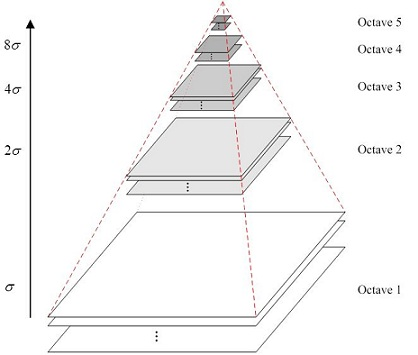
\includegraphics{gausspy}
\caption{图像的一组高斯金字塔}
\label{fig:gausspy}
\end{figure}

高斯金字塔是尺度空间的表示,sift算法是基于尺度空间理论的。尺度空间思想最早是由Iijima\upcite{Iijima}于1962年提出的,后经witkin\upcite{Witkin}和Koenderink\upcite{Koenderink}等人的推广逐渐得到关注,在计算机视觉邻域使用广泛。尺度空间理论的基本思想是:在图像信息处理模型中引入一个被视为尺度的参数,通过连续变化尺度参数获得多尺度下的尺度空间表示序列,对这些序列进行尺度空间主轮廓的提取,并以该主轮廓作为一种特征向量,实现边缘、角点检测和不同分辨率上的特征提取等。尺度理论的数学表达式如公式~\ref{chidu}所示:
\begin{equation}\label{chidu}
L(x,y,\delta)=G(x,y,\delta)*I(x,y)
\end{equation}

其中,*表示卷积运算,G(x,y,$\delta$)为高斯函数,
\begin{equation}\label{gauss}
G(x,y,\delta)=\frac{1}{2\pi{\delta}^2}e^{-\frac{(x-m/2)^2+(y-n/2)^2}{2\delta^2}}
\end{equation}

其中,m和n表示高斯模板的维度,(x,y)代表图像的像素位置,$\delta$是尺度空间因子,值越小表示图像被平滑的越少,相应的尺度也就越小。大尺度对应于图像的概貌特征,小尺度对应于图像的细节特征。

\item 高斯差分金字塔建立\\高斯差分金子塔是在高斯金子塔的基础上的到得,通过将同一组中的相邻层数的高斯图像相减,可以得到高斯差分图像,具体如图~\ref{fig:gaussDog}所示:
\begin{figure}[htp]
\centering
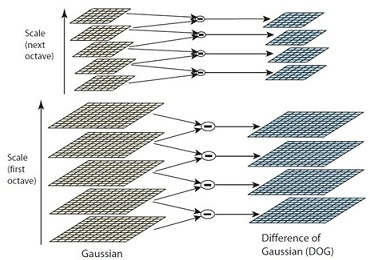
\includegraphics{gaussDog}
\caption{高斯差分金子塔}
\label{fig:gaussDog}
\end{figure}

尺度归一化的高斯拉普拉斯函数${\delta}^2{\nabla}^2{G}$的极大值和极小值同其它的特征提取函数,例如:梯度,Hessian或Harris角特征比较,能够产生最稳定的图像特征。而高斯差分函数(Difference of Gaussian ,简称DOG算子)与尺度归一化的高斯拉普拉斯函数${\delta}^2{\nabla}^2{G}$,它们的关系推导如下:
\begin{equation}\label{dog_1}
\frac{\partial{x}}{\partial{\delta}}=\delta\nabla^2G
\end{equation}

利用差分近似代替微分,则有:
\begin{equation}\label{dog_2}
\delta\nabla^2G=\frac{\partial{x}}{\partial{\delta}}\approx\frac{G(x,y,k\delta)-G(x,y,\delta)}{k\delta-\delta}
\end{equation}

因此就有:
\begin{equation}\label{dog_3}
G(x,y,k\delta)-G(x,y,\delta)\approx(k-1)\delta^2\nabla^2G
\end{equation}

其中k-1是常数,并不影响极值点的位置求取,两者极值关系如图~\ref{fig:py_dog}所示,其中横坐标为0处,最下方的曲线为高斯差分算子,上方为高斯拉普拉斯算子:
\begin{figure}[htp]
\centering
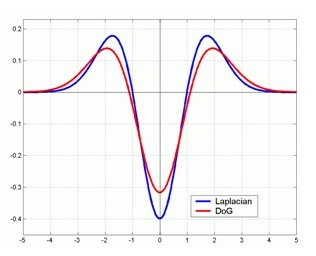
\includegraphics{py_dog}
\caption{高斯拉普拉斯和高斯差分极值关系对比}
\label{fig:py_dog}
\end{figure}

当使用高斯差分算子代替拉普拉斯算子进行极值检测,公式如下所示:
\begin{equation}\label{dog_detect}
D(x,y,\delta)=\Bigl(G(x,y,k\delta)-G(x,y,\delta)\Bigr)*I(x,y)=L(x,y,k\delta)-L(x,y,\delta)
\end{equation}

在实际计算时,使用高斯金字塔每组中相邻上下两层图像相减,得到高斯差分图像,然后在差分图像上进行极点检测。
\item 极点检测\\关键点是由DOG空间的局部极值点组成的,关键点的初步探查是通过同一组内各DoG相邻两层图像之间比较完成的。为了寻找DoG函数的极值点,每一个像素点要和它所有的相邻点比较,看其是否比它的图像域和尺度域的相邻点大或者小。如图3.4所示,中间的检测点和它同尺度的8个相邻点和上下相邻尺度对应的9×2个点共26个点比较,以确保在尺度空间和二维图像空间都检测到极值点。具体如图~\ref{fig:pole_detect}所示:
\begin{figure}[htp]
\centering
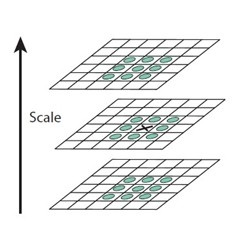
\includegraphics{pole_detect}
\caption{高斯差分图像上的极点检测}
\label{fig:pole_detect}
\end{figure}

\item 关键点精确定位\\离散空间的极值点并不是真正的极值点,图~\ref{fig:keypoint_detect}显示了二维函数离散空间得到的极值点与连续空间极值点的差别。利用已知的离散空间点插值得到的连续空间极值点的方法叫做子像素插值(Sub-pixel Interpolation)。
\begin{figure}[htp]
\centering
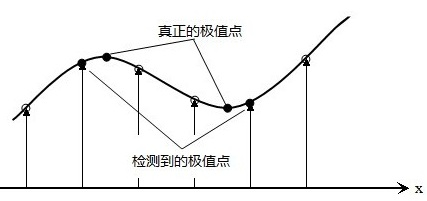
\includegraphics{keypoint_detect}
\caption{离散空间与连续空间极值点的差别}
\label{fig:keypoint_detect}
\end{figure}

为了提高关键点的稳定性,需要对尺度空间DoG函数进行曲线拟合。利用DoG函数在尺度空间的Taylor展开式(拟合函数)如公式~\ref{Tayor},其中$X={(x,y,\delta)^T}$代表相对插值中心的偏移量,当它在任一维度上的偏移量大于0.5时(即x或y或$\delta$),意味着插值中心已经偏移到它的邻近点上,所以必须改变当前关键点的位置,同时在新的位置上反复插值直到收敛,但是此过程有可能超出设定测迭代次数或者图像边界范围,那么这样的点就应该被删除掉,在Lowe的论文中,迭代的上限为5。另外,${|D(x)|}$的值过小会受到噪声影响而变得不稳定,因此该值小于某个阈值的极值点也要删除,在Lowe论文中,使用阈值的大小为0.03。
\begin{equation}\label{Tayor}
D(X)=D+\frac{\partial{D}^T}{\partial{X}}X+\frac{1}{2}X^T\frac{\partial^2{D}}{\partial{X}^2}X
\end{equation}

\item 关键点方向分配和描述\\为了使描述符具有旋转不变性,需要利用图像的局部特征为给每一个关键点分配一个基准方向。使用图像梯度的方法求取局部结构的稳定方向。对于在DOG金字塔中检测出的关键点点,采集其所在高斯金字塔图像3σ邻域窗口内像素的梯度和方向分布特征。梯度的模值和方向如下:
\begin{equation}\label{mozhi}
m(x,y)=\sqrt{L(x+1,y)-{L(x-1,y)}^2+L(x,y+1)-{L(x,y-1)}^2}
\end{equation}
\begin{equation}\label{fangxiang}
\theta(x,y)=\tan^{-1}\Bigl({\frac{L(x,y+1)-L(x,y-1)}{L(x+1,y-L(x-1,y)}}\Bigr)
\end{equation}
\end{compactenum}

其中,L为关键点所在尺度的空间值,邻域窗口半径为3*1.5${\delta}$。

在完成关键点的梯度计算后,使用直方图统计邻域内像素的梯度和方向。梯度直方图将0~360度的方向范围分为36个柱(bins),其中每柱10度。如图~\ref{fig:direct_histogram}所示,直方图的峰值方向代表了关键点的主方向,(为简化,图中只画了八个方向的直方图)。方向直方图的峰值则代表了该特征点处邻域梯度的方向,以直方图中最大值作为该关键点的主方向。为了增强匹配的鲁棒性,只保留峰值大于主方向峰值80%的方向作为该关键点的辅方向。因此,对于同一梯度值的多个峰值的关键点位置,在相同位置和尺度将会有多个关键点被创建但方向不同。仅有15%的关键点被赋予多个方向,但可以明显的提高关键点匹配的稳定性。
\begin{figure}[htp]
\centering
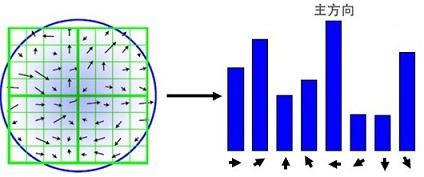
\includegraphics{direct_histogram}
\caption{关键点方向直方图}
\label{fig:direct_histogram}
\end{figure}

在关键点方向被确定之后,我们需要给这些关键点建立一个定量的描述,该描述子不仅包括关键点的信息,也包含关键点周围对其有贡献的像素点,并且描述符应该有较高的独特性,以便于提高特征点正确匹配的概率。SIFT算法中通过一组向量将关键点的特征描述出来,SIFT描述子是关键点邻域高斯图像梯度统计结果的一种表示。通过对关键点周围图像区域分块,计算块内梯度直方图,生成具有独特性的向量,这个向量是该区域图像信息的一种抽象,具有唯一性。

Lowe在论文中建议使用在关键点尺度空间内4*4的窗口中计算的8个方向的梯度信息,共4*4*8=128维向量表征,具体表示步骤如下:
\begin{itemize}
\item 确定计算描述子所需的图像区域
\item 将坐标轴旋转为关键点的方向,以确保旋转不变性
\item 将邻域内的采样点分配到对应的子区域内,将子区域内的梯度值分配到8个方向上,计算其权值
\item 插值计算每个种子点八个方向的梯度
\item 描述子向量门限
\item 按特征点的尺度对特征描述向量进行排序
\end{itemize}

至此,SIFT特征描述向量生成完毕。

在上述5个步骤中,构建高斯金字塔和极点检测是最为耗时的两个。构建高斯金字塔时需要对每张图片进行高斯滤波,高斯滤波是一个时间复杂度为O(N3) 的操作,这里的N与图像大小成正比。图~\ref{fig:gausspy}中仅显示了一组金字塔,而SIFT算法往往需要构建多组金字塔,使得构建高斯金字塔的时间复杂度达到O(O*I*N3),其中O为高斯塔的组数,I为高斯塔的层数。极点检测则是在整个金字塔组上进行的,相当于在一个维度为4的空间(组,层,长,宽)中搜索极值点,它的时间复杂度为O(O*I*N2)。SIFT算法流程中既包含高斯滤波和图像缩放等通用性较强的操作,也含有构建高斯(查分)金字塔、极点检测、消除边缘响应等通用性较差的操作。它的空间复杂度和时间复杂度都比较高,当有海量的图片需要进行特征提取时,占用内存较多,所需的处理时间也会很长。这也是我们使用Spark去加速SIFT算法的原因。

只有充分理解SIFT算法原理之后,才能比较好的在Spark上实现大规模特征提取工作。

\section{Spark核心技术原理}
在这一小节中,将会对Spark中三个核心技术原理进行分析,它们分别是内存编程原理,任务调度原理,性能优化。这三个技术在本文的设计起非常重要的地位,只有将这些技术理解透彻后,才能自如的解决开发过程中遇到的问题。
\subsection{Spark内存编程原理}
Spark区别于其他的大数据处理框架,比如Hadoop\upcite{Hadoop},在于它是一个内存计算的大数据处理框架,它可以将处理的中间结果保存在内存中,后续的计算可以在此基础上直接运行,提升了执行的效率。那么,这么多的数据保存在内存中,这就必须基于分布式内存的数据结构抽象,让开发人员基于该数据结构进行操作,只要操作这些数据,它们就是位于集群的内存中的。上面说的内存抽象数据结构就是RDD(Resilient Distributed Dataset弹性分布式数据集),RDD是Spark最核心的概念,接下来将从RDD的底层实现原理,RDD的操作类型,RDD的缓存原理,RDD 的依赖关系和DAG的生成这几方面分析RDD。
\subsubsection{RDD的底层实现原理}
RDD的基本单元是分区(Partition),一个RDD由多个分区组成,每个分区都会被逻辑映射成一个Block,一个Block会被一个Task执行,这些Block由BlockManager管理,BlockManager负责管理这些Block在集群内的分布。整个过程如图~\ref{fig:blockmanager}所示:
\begin{figure}[htp]
\centering
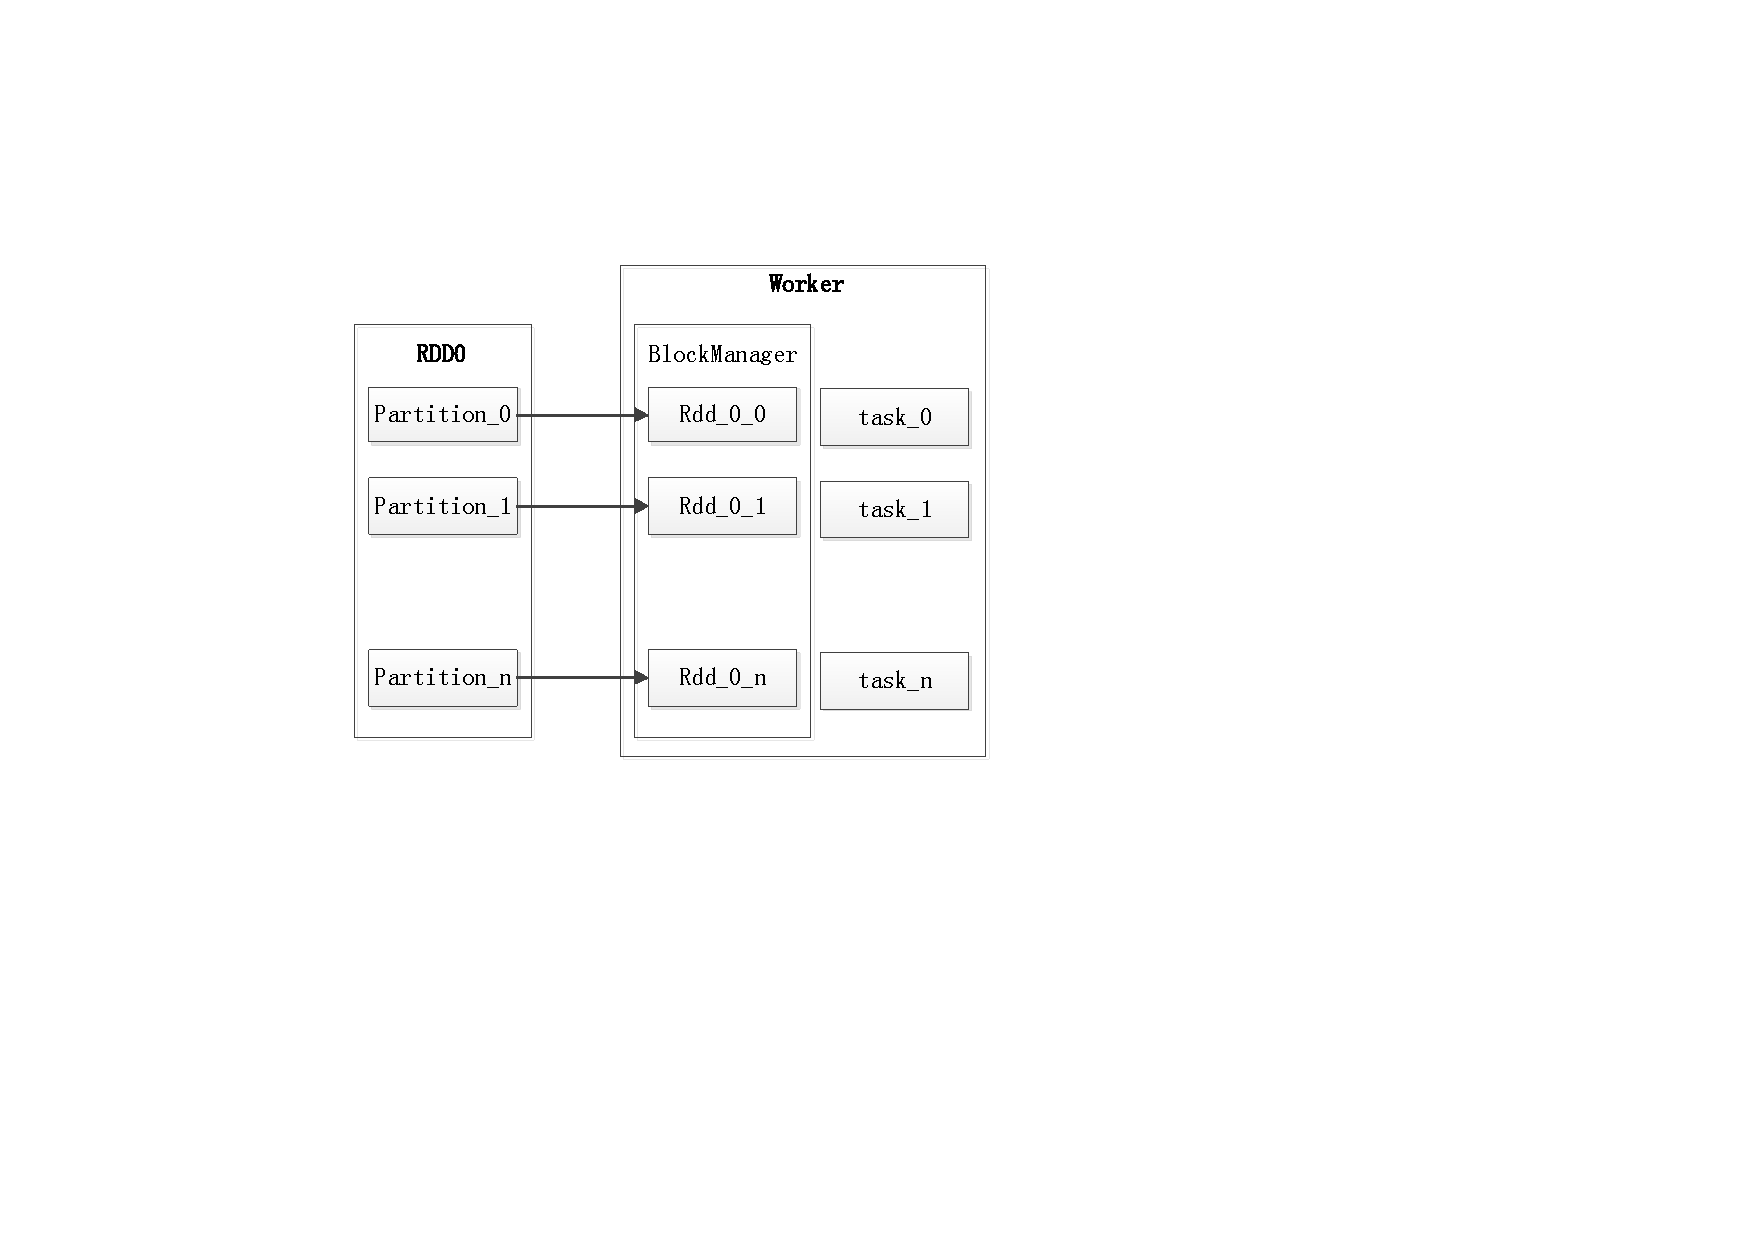
\includegraphics{blockmanager}
\caption{RDD Partition的存储和计算模型}
\label{fig:blockmanager}
\end{figure}

\subsubsection{RDD的操作类型}
RDD提供的操作可以分为两种类型,分别是transformtion(转换)和action(动作),表\ref{tab:trans}和表\ref{tab:action}分别列出了常用的转换操作和动作操作。所有的转换操作都是惰性的,被调用时,它们不会直接计算结果,它们只是记住上一个转换动作,当一个动作操作被调用时,这些转换操作才会被执行。这种设计会让Spark运行得更加高效率,因为可能在动作操作时,被操作的数据集会变得比较小。
\begin{table}[h] %开始一个表格environment,表格的位置是h,here。
\caption{RDD转换操作} %显示表格的标题
\centering
\label{tab:trans}
\begin{tabular}{p{6cm}|p{8cm}} %设置了每一列的宽度,强制转换。
\hline
\hline
转换  & 含义 \\ %用&来分隔单元格的内容 \\表示进入下一行
\hline %画一个横线,下面的就都是一样了,这里一共有4行内容
map(func)  & 返回一个新的分布式的数据集,该数据集有每一个输入元素经过func函数转换后组成\\
\hline
filter(func)  & 返回一个新的数据集,该数据集经过func函数计算后返回值为true的输入元素组成\\
\hline
flatMap(func)  & 类似于Map,但是每一个输入元素可以被映射为0个或者是多个输出元素\\
\hline
mapPartitions(func) & 类型于map,但是独立在RDD的每一个分片上运行,因此func的类型必须是Iterator[T]=>Iterator[U]\\
\hline
mapPartitionWithSplit(func) & 类似于mapPartitions,但是func带有一个整型参数表示分片的索引值,func的函数类型为(Int,Iterator[T])=>Iterator[U]\\
\hline
sample(withReplacement,fraction,seed) & 根据fraction指定比例对数据进行采用\\
\hline
union(otherDataset) & 返回一个新的数据集,新数据集是由源数据集和参数数据集联合而成的\\
\hline
distinct(numTasks) & 返回一个包含源数据集中所有不重复的元素的新的数据集\\
\hline
\hline
\end{tabular}
\end{table}

\begin{table}[h] %开始一个表格environment,表格的位置是h,here。
\caption{RDD动作操作} %显示表格的标题
\centering
\label{tab:action}
\begin{tabular}{p{6cm}|p{8cm}} %设置了每一列的宽度,强制转换。
\hline
\hline
动作  & 含义 \\ %用&来分隔单元格的内容 \\表示进入下一行
\hline %画一个横线,下面的就都是一样了,这里一共有4行内容
reduce(func)  & 通过函数func聚集数据集中的所有元素\\
\hline
collect()  & 在驱动程序中,以数组的形式返回数据集中的所有元素。通常在使用filter或者其他操作返回一个足够小的数据子集后再使用比较有用\\
\hline
count()  & 返回数据集的个数\\
\hline
first() & 返回数据集的第一个元素\\
\hline
take(n) & 返回一个由数据集的前n个元素组成的数组\\
\hline
takeSample(withReplacement,num,seed) & 返回一个数组,该数组由从数据集中随机采用的num个元素组成\\
\hline
saveAsTextFile(path) & 将数据集的元素以textFile的形式保存到本地文件系统,HDFS或者任何Hadoop支持的文件系统\\
\hline
saveAsSequenceFile(path) & 将数据集的元素以Hadoop sequencefile的格式保存到指定目录下,可以是本地系统,HDFS或者任何Hadoop支持的文件系统\\
\hline
countByKey() & 对(K,V)类型的RDD有效,返回一个(K,Int)对的map,表示每一个key的元素个数\\
\hline
foreach(func) & 在数据集的每一个元素上,运行函数func进行更新\\
\hline
\hline
\end{tabular}
\end{table}

\subsubsection{RDD的缓存原理}
spark速度非常快的原因之一,就是在不同操作中内存中持久化(或缓存)一个数据集。当持久化一个RDD后,每一个节点都将会把计算分片的结果保存在内存中,后续的其他操作可以直接使用该结果,这就使得后续的动作变得十分迅速。

通过persist()或cache()方法可以标识一个要被持久化的RDD,一旦首次被触发后,该RDD将会被保留在计算节点的内存中并重用。persist()和cache()的实现如下:
\begin{lstlisting}[language=Java,numbers=none,frame=none]
/**Persist this RDD with the default storage level('MEMORY_ONLY').*/
def persist(): this.type = persist(StorageLevel.MEMORY_ONLY)
/**Persist this RDD with the default storage level('MEMORY_ONLY').*/
def cache(): this.type = persist()
\end{lstlisting}

假设首先进行了RDD0$\rightarrow$RDD1$\rightarrow$RDD2的计算作业,如果RDD1已经被缓存在内存中,那么后续在进行RDD0$\rightarrow$RDD1$\rightarrow$RDD3的计算作业时,就不需要从头开始,直接从RDD1往下执行作业即可,因此计算速度得到了很大的提升,具体过程如下图\ref{fig:rdd_cache}所示:
\begin{figure}[htp]
\centering
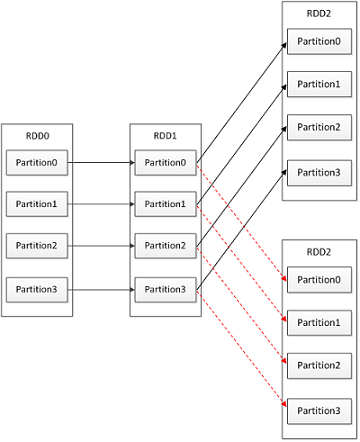
\includegraphics{rdd_cache}
\caption{RDD 缓存加速原理}
\label{fig:rdd_cache}
\end{figure}

缓存的rdd有可能会丢失,或者因为内存不足而删除,但是rdd有完整的容错机制,保证在rdd丢失或者删除的情况下计算依然可以正确执行。
\subsubsection{RDD的依赖关系和DAG的生成}
一个Spark应用中,不同的RDD间存在依赖关系,依赖关系分为窄依赖(narrow dependency)和宽依赖(wide dependency),窄依赖和宽依赖的定义如下:
\begin{itemize}
\item 窄依赖,窄依赖是指父RDD的每个分区只被子RDD的一个分区所使用,如图\ref{fig:dependency}左边部分显示
\item 宽依赖,宽依赖是指父RDD的每个分区都可能被多个子RDD分区所使用,如图\ref{fig:dependency}右边部分显示
\end{itemize}
\begin{figure}[htp]
\centering
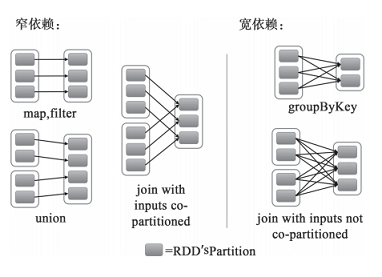
\includegraphics{dependency}
\caption{RDD窄依赖和宽依赖对比}
\label{fig:dependency}
\end{figure}
在Spark应用开发中,RDD会经过很多转换操作,每个转换操作都会生成一个新的RDD,这些转换操作最后会形成一个有向图(Directed Acyclic Graph,简称DAG)。这个DAG记录着RDD间的依赖关系,借助这些依赖关系,能保证一个RDD被计算前,所有它所依赖的parent RDD都已经完成了计算。同时Spark 也是整个DAG根据依赖关系的不同划分为不同的阶段(stage),一个stage中包含的一组并行执行的任务。划分stage的依据是,rdd间是窄依赖关系的划分到一个stage中,rdd间是宽依赖的划分到不同的stage中。一个stage中可以并行执行,不同stage 间顺行执行。
\subsection{Spark任务调度原理}
Spark任务调度框架主要由三个模块支撑起,它们分别是DAGScheduler,SchedulerBackend及TaskScheduler。首先DAGScheduler分析用户提交的应用,根据依赖关系建立DAG,然后将DAG 划分为不同的Stage,而stage中包含所要执行的tasks。SchedulerBackend负责整个集群交互,收集可用的资源信息,然后将这些信息上报TaskScheduler。TaskScheduler将从SchedulerBackend获取到的资源信息以及从DAGScheduler生成的tasks进行一个资源的分配,将tasks分配的合适的资源上面。整个流程如图\ref{fig:schedulerfw}所示:
\begin{figure}[htp]
\centering
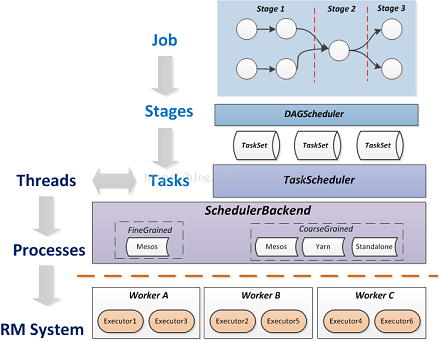
\includegraphics{schedulerfw}
\caption{Spark任务调度框架}
\label{fig:schedulerfw}
\end{figure}
\subsubsection{DAGScheduler}
DAGScheduler面向stage的调度(stage-oriented scheduling)的高级调度器,将job根据类型划分为不同的stage(划分的依据是依赖关系为窄依赖的属于一个stage,依赖关系为宽依赖的RDD属于不同的stage)为每个job 的不同stage 计算DAG,跟踪哪些RDD和stage被物化并且发现运行job的最小的调度策略,然后并在每一个stage 内产生一系列的task 并封装为taskset, 结合当前的缓存情况来决定每个Task的最佳位置(任务在数据所在的节点上运行),以taskset 为单位提交(submitTasks) 给TaskScheduler。
\subsubsection{SchedulerBackend}
SchedulerBackend负责与Cluster Manager交互,取得该Application分配到的资源,并且将这些资源传给TaskScheduler,由TaskScheduler为Task最终分配计算资源。在不同的集群模式下,SchedulerBackend的实现是不一样的,实现可以分为细粒度和粗粒度两种。分为细粒度和粗粒度两种。细粒度只有Mesos(mesos有粗细两种粒度的使用方式)实现了,粗粒度的实现者有yarn,mesos,standalone。拿standalone模式来说粗粒度,每台物理机器是一个worker,worker一共可以使用多少cpu和内存,启动时候可以指定每个worker起几个executor,即进程,每个executor的cpu和内存是多少。粗粒度与细粒度的主要区别,就是粗粒度是进程long-running 的,计算线程可以调到executor上跑,但executor的cpu和内存更容易浪费。细粒度的话,可以存在复用,可以实现抢占等等更加苛刻但促进资源利用率的事情。这俩概念还是AMPLab论文里最先提出来并在Mesos里实现的。AMPLab在资源使用粒度甚至任务分配最优的这块领域有不少论文,包括Mesos的DRF算法、Sparrow调度器等。所以standalone模式下,根据RDD的partition数,以及每个task需要的cpu 数,可以很容易计算每台物理机器的负载量、资源的消耗情况、甚至知道TaskSet要分几批才能跑完一个stage。
\subsubsection{TaskScheduler}
TaskScheduler负责Application的不同Job间的调度,在Task执行失败时启动重试机制。TaskScheduler里会对已经提交的tasks进行一次优先级排序,这个排序策略目前有两种:FIFO(First In First Out,先进先出)或FAIR(公平调度),默认调度策略是FIFO。通过排序,会得到一份待运行的tasks,然后就把从schedulerBackend交过来的worker资源信息合理分配给这些tasks。分配前,为了避免每次都是前几个worker被分到tasks,所以先对WorkerOffer列表进行一次随机洗牌。接下来就是遍历tasks,看workers的资源“够不够”,“符不符合”task,如果符合的话task就被正式launch起来。
\subsection{Spark性能优化原理}
在本小节中,将介绍Spark的性能优化原理,因为Spark是处理大数据的框架,因此性能优化是非常有必要的。接下来将从几个方面分析spark的性能问题
\subsubsection{调度和分区优化}
在spark应用程序中,会经常使用fiter算子进行数据过滤,而频繁的过滤或者过滤的数据量过大就会造成大量小分区,由于spark是每个数据分区都会分配一个任务执行,如果任务过多,就会造成线程切换开销很大,很多任务等待执行,并行度实际上不高。面对这种情况,我们可以采用RDD中的重分区函数进行数据的紧缩,减少分区数,将小分区合并成大分区。具体可以通过coalesce函数进行,函数定义如下:
\begin{lstlisting}[language=Java,numbers=none,frame=none]
def coalesce(numPartitions: Int, shuffle: Boolean = false)(implicit ord: Ordering[T] = null): RDD[T]
\end{lstlisting}

该函数会返回一个含有numPartitions数量个分区的新的RDD,即将整个RDD重分区。

使用这个函数会出现一个问题,比如将1000个分区的RDD重分区为一个分区,就会造成数据过于集中,完成无法开掘集群并行计算的能力。在这种情况下,可以将coalsesce 函数参数shuffle 设置为true,由于shuffle 可以分隔shuffle,这就保证了上游的任务仍是1000个,否则两个上下游的任务合并为一个stage 计算,这个stage就会在一个分区上进行并行计算。

除了将分区收缩,在某些情况下,可能会对原来的分区进行扩充,将分区数量增加,以利用并行计算能力。在这个过程中,默认使用的是Hash分区器进行重分区。

在分区优化问题中,还有一个倾斜(skew)的问题。倾斜是一个大数据处理中一个非常重要的问题,可以分为数据倾斜和任务倾斜,数据倾斜的结果就会造成任务倾斜,在个别分区上,任务的执行时间过长。
\begin{compactenum}
\item 数据倾斜\\产生数据倾斜的原因大致有这几种:
\begin{itemize}
\item key数据分布不均匀,因为spark中默认是按照Hash方式进行分区,如果某个key的数据特别多,就会造成分到某个key上的数据特别多,最后造成某个分区的数据特别多,也就出现了数据倾斜。
\item 结构化数据表设计问题
\item 某些SQL语句产生数据倾斜
\end{itemize}

\item 任务倾斜\\产生任务倾斜的原因较为隐蔽,有可能是服务器架构的原因,有可能是JVM的原因,有可能是线程池的原因,也有可能是业务本省的原因。比如在本文设计中就发现,即使是两个任务的处理数据的总大小一样,但是仍然会产生任务倾斜,这和处理问题的具体场景有关系,在SIFT算法中,算法的时间复杂度和图片的尺寸大小有关系的。
\end{compactenum}

\subsubsection{内存存储优化}
因为spark是内存计算的大数据处理框架,因此内存存储优化也是十分重要的内容。内存调优过程中,有三个方向值得考虑,分别是JVM调优,OOM问题调优及磁盘临时目录空间优化。
\begin{compactenum}
\item JVM调优\\不同的JAVA对象都有一个对象头,这些信息有时候比数据本身的信息还要大,比如只有一个Int属性的对象。还有一些链式结构,它们会包含一些指针信息。因此在开发的过程要选好数据类型和数据结构,尽量减少一些链式结构的使用;减少对象的嵌套;可以考虑使用数字ID或者是枚举对象,而不是字符串作为key的关键数据。
\item OMM问题调优\\在spark开发过程中,内存溢出(OutOfMemoryError)是一个经常会遇到的问题,发生内存溢出的原因是Java虚拟机创建的对象太多,在进行垃圾回收时,虚拟机分配的堆空间已经用满了,与heap space有关。解决这类问题有两种思路,一种是减少App的内存占用空间消耗,另一种是增大内存资源的供应。具体设计时,可以查看程序中是否有循环创建对象的地方,程序中应该减少这种代码的存在,或者可以调整JVM中的Xmx(最大堆)和Xms(最小堆)参数的大小。另外,还要查看在做shuffle类操作符时是否创建的Hash表过大,在这种情况下,可以通过增加任务数,即分区数来提升并行度,减少每个任务的输入数据,减少内存占用来解决问题。
\end{compactenum}

\subsubsection{磁盘临时目录空间优化}
Spark在进行shuffle的过程中,中间结果会写到spark在磁盘的临时目录中,如果临时目录过小的话,会造成No Space left on device异常,在这种情况下可以配置多个盘块来扩展Spark的磁盘临时目录,让更多的数据可以写到磁盘,加快I/O速度。
\subsubsection{网络传输优化}
Spark是大数据处理框架,因此集群中数据传输也是影响应用性能的重要因素。如果可以减少数据传输的次数或者是传输的大小,可能会极大的提高应用的性能。下面将分析spark中数据传输优化的场景。
\begin{compactenum}
\item 大局部变量的传输\\默认情况下,算子函数内,如果使用了外部变量,那么会将这个变量的拷贝到执行这个函数的每一个task中,如果这个变量十分大,比如是一个大数组,而且执行的任务又特别多,那么网络的传输耗费就会特别大。下面就是一个例子的展示,其中factor就是一个变量,它在map任务中被使用:
\begin{lstlisting}[language=Java,numbers=none,frame=none]
val factor = 3
rdd.map(num => num*factor)
\end{lstlisting}

面对这种情况,可以使用Spark的Brodcast(广播)变量对数据传输进行优化,通过Brocast变量将用到的大数据量数据进行广播发送,可以提升整体速度。Broadcast主广播的变量是只读的,并且在每个节点上只会有一份副本,而不会为每个task都拷贝一个副本。因此就减少了变量到各个节点的网络传输消耗,以及在各个节点上的内存消耗。
\item 大结果收集\\在spark的开发中,会经常用到collect操作,collect操作将各个分区的结果收集到一个数组,返回到driver。如图\ref{fig:collect}如果收集的结果过大,就会拖慢应用的执行时间,甚至造成内存溢出。
\begin{figure}[htp]
\centering
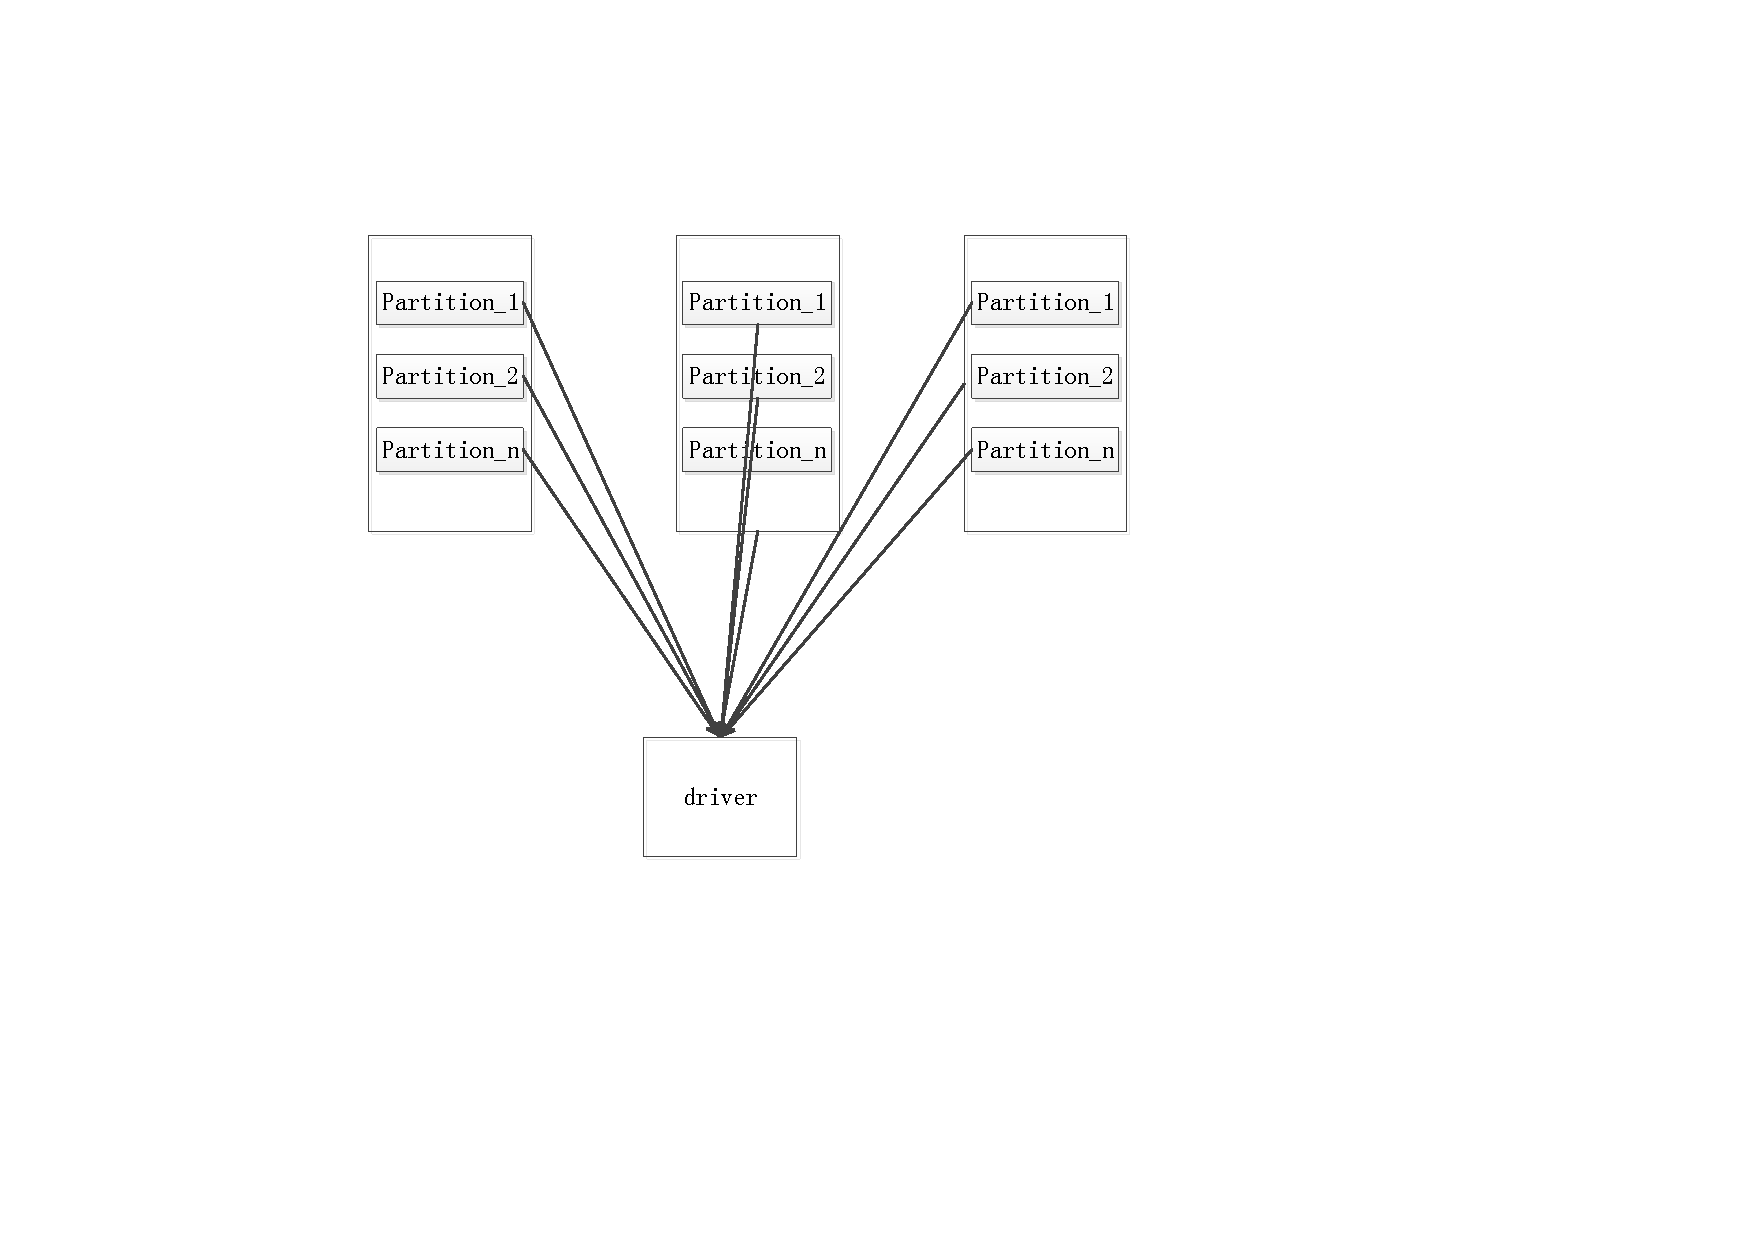
\includegraphics{collect}
\caption{collect操作收集所有分区}
\label{fig:collect}
\end{figure}
面对这种情况,如果收集的结果过大,可以将数据分布式的存储在HDFS或者其他的分布式持久化层上,这样可以减少单机数据的I/O开销和单机内存的存储压力。
%%\subsubsection{序列化与压缩}
\end{compactenum}
\section{分布式存储原理}

\section{GPU特征提取原理}

\section{本章小结}
本章分析了本文工作的一些技术原理,首先分析SIFT算法原理,主要针对SIFT算法的5个主要步骤进行分析,分析其数学原理及作用,然后讨论了算法的时间复杂性。接着介绍了作为本文设计的计算引擎Spark,主要涉及了Spark核心技术原理,主要包括Spark的内存编程原理,任务调度原理,性能优化原理。最后介绍了本文设计中作为存储层的分布式文件系统HDFS的一些核心原理。最后,介绍了作为本文设计的比较的GPU特征提取原理。



\chapter{大规模特征提取系统Spark-SIFT实现}
在本章节中将详细介绍整个大规模特征提取系统Spark-SIFT的设计和实现。首先会介绍系统的整体框架和数据流程,接着会针对系统中的各个模块进行分析,主要包括功能模块,存储模块,容错模块,最后会介绍系统的部署和正确性验证。

\section{系统架构与数据流程}
大规模图像库特征提取系统Spark-SIFT框架图如图\ref{fig:spark_sift_fw}所示:
\begin{figure}[htp]
\centering
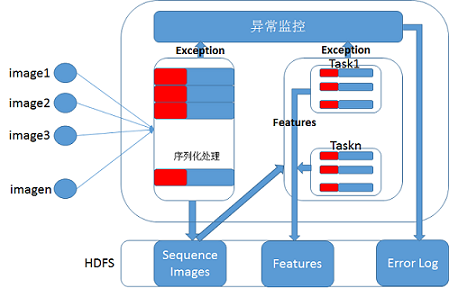
\includegraphics{spark_sift_fw}
\caption{大规模图像库特征提取系统Spark-SIFT系统框架}
\label{fig:spark_sift_fw}
\end{figure}
图像库进行特征提取前,先经过序列化处理模块进行序列化处理,经过序列化模块之后,一张图片转化单条记录的形式,最后所有的记录序列化保存到分布式文件系统HDFS 中。当进行特征提取时,特征提取功能模块读取HDFS中序列化图片记录,将其分发到各个任务上,任务运行在整个集群上,每个任务上通过Spark-SIFT算法进行特征提取,完成特征提取后,每个task 直接将提取出来的特征保存到HDFS中。Spark-SIFT系统中的异常监控模块收集特征提取作业运行过程中出现的异常信息,将异常信息写到特定的异常日志中。

从软件架构的角度看整个系统,系统的框架图如图\ref{fig:spsift_core_fw}所示:
\begin{figure}[htp]
\centering
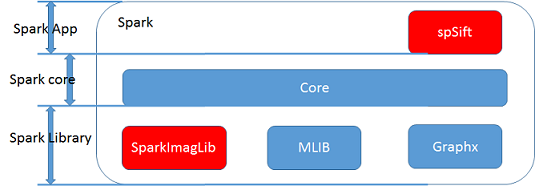
\includegraphics{spsift_core_fw}
\caption{Spark-SIFT软件架构}
\label{fig:spsift_core_fw}
\end{figure}
本文的主要工作在于Spark的库层和应用层。本文实现了Spark下的图像处理基础库Spark-imageLib,这个库包含了spark的图像的表示,读取操作及一些基础的图像处理接口,比如图像的灰度化,图像的缩放,图像的模糊等;这个库和spark的其他库,比如分布式图计算处理库GraphX,机器学习库MLib的地位是等价的,我们已经将该库嵌入到spark的生态系统中。此在这个库的基础上,开发了Spark-SIFT 算法,该算法在Spark 应用中被调用,实现分布式的特征提取工作,图中的spSift 就是特征提取应用,它位于spark 的应用层。
\section{系统模块设计}
在本小节中,会详细介绍每个模块的设计及实现,它们分别是spark图像基础库spark-imageLib,spark-sift算法,序列化模块,存储模块以及系统容错模块。
\subsection{spark图像基础库spark-imageLib}
spark-imageLib图像处理库主要包括图像的表示,图像的读取,特征点的表示。
\subsubsection{图像表示}
在图像表示中,本文设计主要用到了三个类,分别是SpImage,SpSingleBandImage及SpFImage,它们间的继承关系如图\ref{fig:image_represent}:
\begin{figure}[htp]
\centering
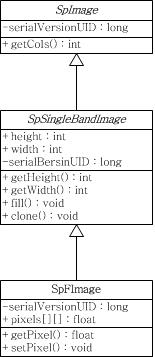
\includegraphics{image_represent}
\caption{Spark下图像表示}
\label{fig:image_represent}
\end{figure}
SpImage为最基础的为抽象类,不会直接被使用。SpSingleBandImage为SpImage的子类,它也为抽象类,SpSingleBandImage表示单通道类型的图像。SpFImage类为SpSingleBandImage的子类,也是本文中实际用来在Spark下表示图像的类。这三个类都有一个共同的属性变量,就是serialVersionUID,因为本文是一个分布式的图像处理框架,必然会设计到处理图像文件的网络传输,因此表示图像的类必须是序列化的,这样才能使得图像可以在Spark这个分布式框架下处理。这里的序列化采用的java的序列化方式,因为序列化必然会存在一个反序列化的过程,比如从Master 将图像序列化传送的Worker上,然后Worker 将接受到的内容反序列化得到原始图像,为了避免两端实体类的内容不一样,就使用了serialVersionUID 作为衡量的标准。当JVM获取传来的字节流时,先读取serialVersionUID,然后和本地的进行比较,根据比较的结果判断是否可以进行序列化。

考虑传输过程中的耗费代价,因此设计SpFImage数据结构时要十分精简,在成员变量中,只设置了一个二维数组pixels,这个数组就是保存整张图片的像素信息。因为考虑到高斯模糊时候的精度问题,所以pixels采用了float类型。SpFImage的构造函数是比较灵活的,它允许传递一维数组或者是二维数组,数组的类型是byte或者float,对于不同的参数类型,本文都会自动进行转换。

表\ref{tab:SpFImage_function}列出三个类的主要功能函数:
\begin{table}[h] %开始一个表格environment,表格的位置是h,here。
\caption{SpFImage 主要功能函数} %显示表格的标题
\centering
\label{tab:SpFImage_function}
\begin{tabular}{p{4cm}|p{2cm}|p{6cm}} %设置了每一列的宽度,强制转换。
\hline
\hline
函数名  & 所属类 & 功能 \\ %用&来分隔单元格的内容 \\表示进入下一行
\hline %画一个横线,下面的就都是一样了,这里一共有4行内容
abs  & SpFImage & 对图片的像素点进行绝对值操作\\
\hline
addInplace  & SpFImage & 将图片的像素进行加操作\\
\hline
subtractInplace  & SpFImage & 将图片的像素进行减操作\\
\hline
multiplyInplace  & SpFImage & 将图片的像素进行乘操作\\
\hline
divideInplace  & SpFImage & 将图片的像素进行乘操作\\
\hline
fill  & SpFImage & 对图片进行填充操作\\
\hline
getDoublePixelVector & SpFImage & 将图片像素以一维向量的形式返回\\
\hline
getPixel& SpFImage & 获取图片某个位置上的像素值\\
\hline
setPixel & SpFImage & 对图片某个位置的像素进行赋值\\
\hline
threshold & SpFImage & 对图片像素进行阈值判断\\
\hline
\hline
\end{tabular}
\end{table}
\subsubsection{图像的读取}
在图片读取这个模块中,主要使用到SpImageUtilities类型,该类提供了从字节流到SpFImage的转换接口,该类的主要成员函数表\ref{tab:SpImageUtilities_function}所示:
\begin{table}[h] %开始一个表格environment,表格的位置是h,here。
\caption{SpImageUtilities 主要功能函数} %显示表格的标题
\centering
\label{tab:SpImageUtilities_function}
\begin{tabular}{p{3cm}|p{3cm}|p{6cm}} %设置了每一列的宽度,强制转换。
\hline
\hline
函数名  & 所属类 & 功能 \\ %用&来分隔单元格的内容 \\表示进入下一行
\hline %画一个横线,下面的就都是一样了,这里一共有4行内容
readF  & SpImageUtilities & 将字节流转化成SpFImage\\
\hline
createFImge  & SpImageUtilities & 将BufferedImage类型的图片转换成SpFImage类型\\
\hline
createBufferImage & SpImageUtilities & 将SpFImage类型图片转换成BufferImage图片\\
\hline
checkSize  & SpImageUtilities & 对图片的大小进行检查\\
\hline
\hline
\end{tabular}
\end{table}

因为图片库是保存在HDFS中的,因此需要用特定的HDFS接口进行读取,在读取完之后在使用SpImageUtilities接口进行转换。在HDFS读取接口中,可以通过三个接口进行图片的读取,它们分别是,sequenceFile,binaryFiles及objectFile函数。sequenceFile是spark下用来读取序列化文件的接口,具体定义如下:
\begin{lstlisting}[language=Java,numbers=none,frame=none]
def sequenceFile[K,V](path:String,KeyClass:Class[K],valueClass:Class[V],minPartitions:Int):RDD[(K,V)]=withScope{}
\end{lstlisting}
sequenceFile保存的是Writable,换句话讲,key和value也必须是Writable类型的,表\ref{tab:Writable}列出了常见类型的Writable对应类型。
\begin{table}[h] %开始一个表格environment,表格的位置是h,here。
\caption{Writable对应类型} %显示表格的标题
\centering
\label{tab:Writable}
\begin{tabular}{p{4cm}|p{2cm}|p{6cm}} %设置了每一列的宽度,强制转换。
\hline
\hline
Scala类型  & Java类型 & Writable类型 \\ %用&来分隔单元格的内容 \\表示进入下一行
\hline %画一个横线,下面的就都是一样了,这里一共有4行内容
Int  & Integer & IntWritable\\
\hline
Long  & Long & LongWritable\\
\hline
Float  & Float & FloatWritable\\
\hline
Double  & Double & DoubleWritable\\
\hline
Array[Byte]  & byte[] & BytesWritable\\
\hline
String  & String & Text\\
\hline
List[T] & List<T> & ArrayWritable\\
\hline
Array[T] & T[] & ArrayWritable\\
\hline
\hline
\end{tabular}
\end{table}

本文设计中,采用sequenceFile读取图片的主要代码如下:
\begin{lstlisting}[language=Java,numbers=none,frame=none]
val fn_rdd = sc.sequnceFile(imageSEQ_path,classOf[Text],classOf[BytesWritable],task_size.toInt)
.map({case (fname,fcon)} => {
  var datainput:InputStream = new ByteArrayInputStream(fcontext.getBytes)
  var img = SpImageUtilities.readF(datainput)//读取图片的像素矩阵
...
})
\end{lstlisting}
采用binaryFiles接口进行读取时,返回的是(String,PortableDataStream)类型的RDD,binaryFiles的定义如下:
\begin{lstlisting}[language=Java,numbers=none,frame=none]
def binaryFiles(path:String,minPartitions:Int = defaultMinPartitions):RDD[(String,PortableDataStream)]=withScope{}
\end{lstlisting}
使用binaryFiles接口读取图像的主要代码如下:
\begin{lstlisting}[language=Java,numbers=none,frame=none]
 sc.binaryFiles(initImgs_path_hdfs,task_size.toInt).map(f => {
      val fname = new Text(f._1.substring(prefix_path_hdfs.length,f._1.length))//获取features key
      val bytes = f._2.toArray()

      var datainput:InputStream = new ByteArrayInputStream(bytes)
      var img = SpImageUtilities.readF(datainput)
      ...
}
)
\end{lstlisting}
objectFile读取的是对象文件,保存的时候以什么对象类型保存,就以什么类型读取读出,该函数看似对SequenceFile的简单封装,它运行存储只包含值的RDD,两者的区别在于objectFile保存对象时是采用java序列化的方式,SequenceFile采用的则是hadoop的序列化方式。 objectFile 函数定义如下:
\begin{lstlisting}[language=Java,numbers=none,frame=none]
def objectFile(path:String,minPartitions:Int = defaultMinPartitions):RDD[T]=withScope{}
\end{lstlisting}
使用objectFile接口读取图像的主要代码如下:
\begin{lstlisting}[language=Java,numbers=none,frame=none]
sc.objectFile(initImgs_500k_path_hdfs).map(x => {
    val test:SpFImage = x
    ...
})
\end{lstlisting}
虽然objectFile读取图像十分方便,但是如果直接将对象保存到HDFS中,储存空间相当大,存储的时间也十分长。
\subsubsection{特征点表示}
%%加上序列化的内容,Hadoop下怎样序列化
在本文设计中,特征点的表示只要涉及到三个模块,分别是SpKeypoint,SpMemoryLocalFeatureList,SpLocalFeatureList。SpKeypoint表示一个sift特征点,SpMemoryLocalFeatureList保存整张图片的sift 特征点,SpLocalFeatureList为接口,SpMemoryLocalFeatureList是SpLocalFeatureList的具体实现。SpKeypoint成员结构如图\ref{fig:spkeypoint}所示:
\begin{figure}[htp]
\centering
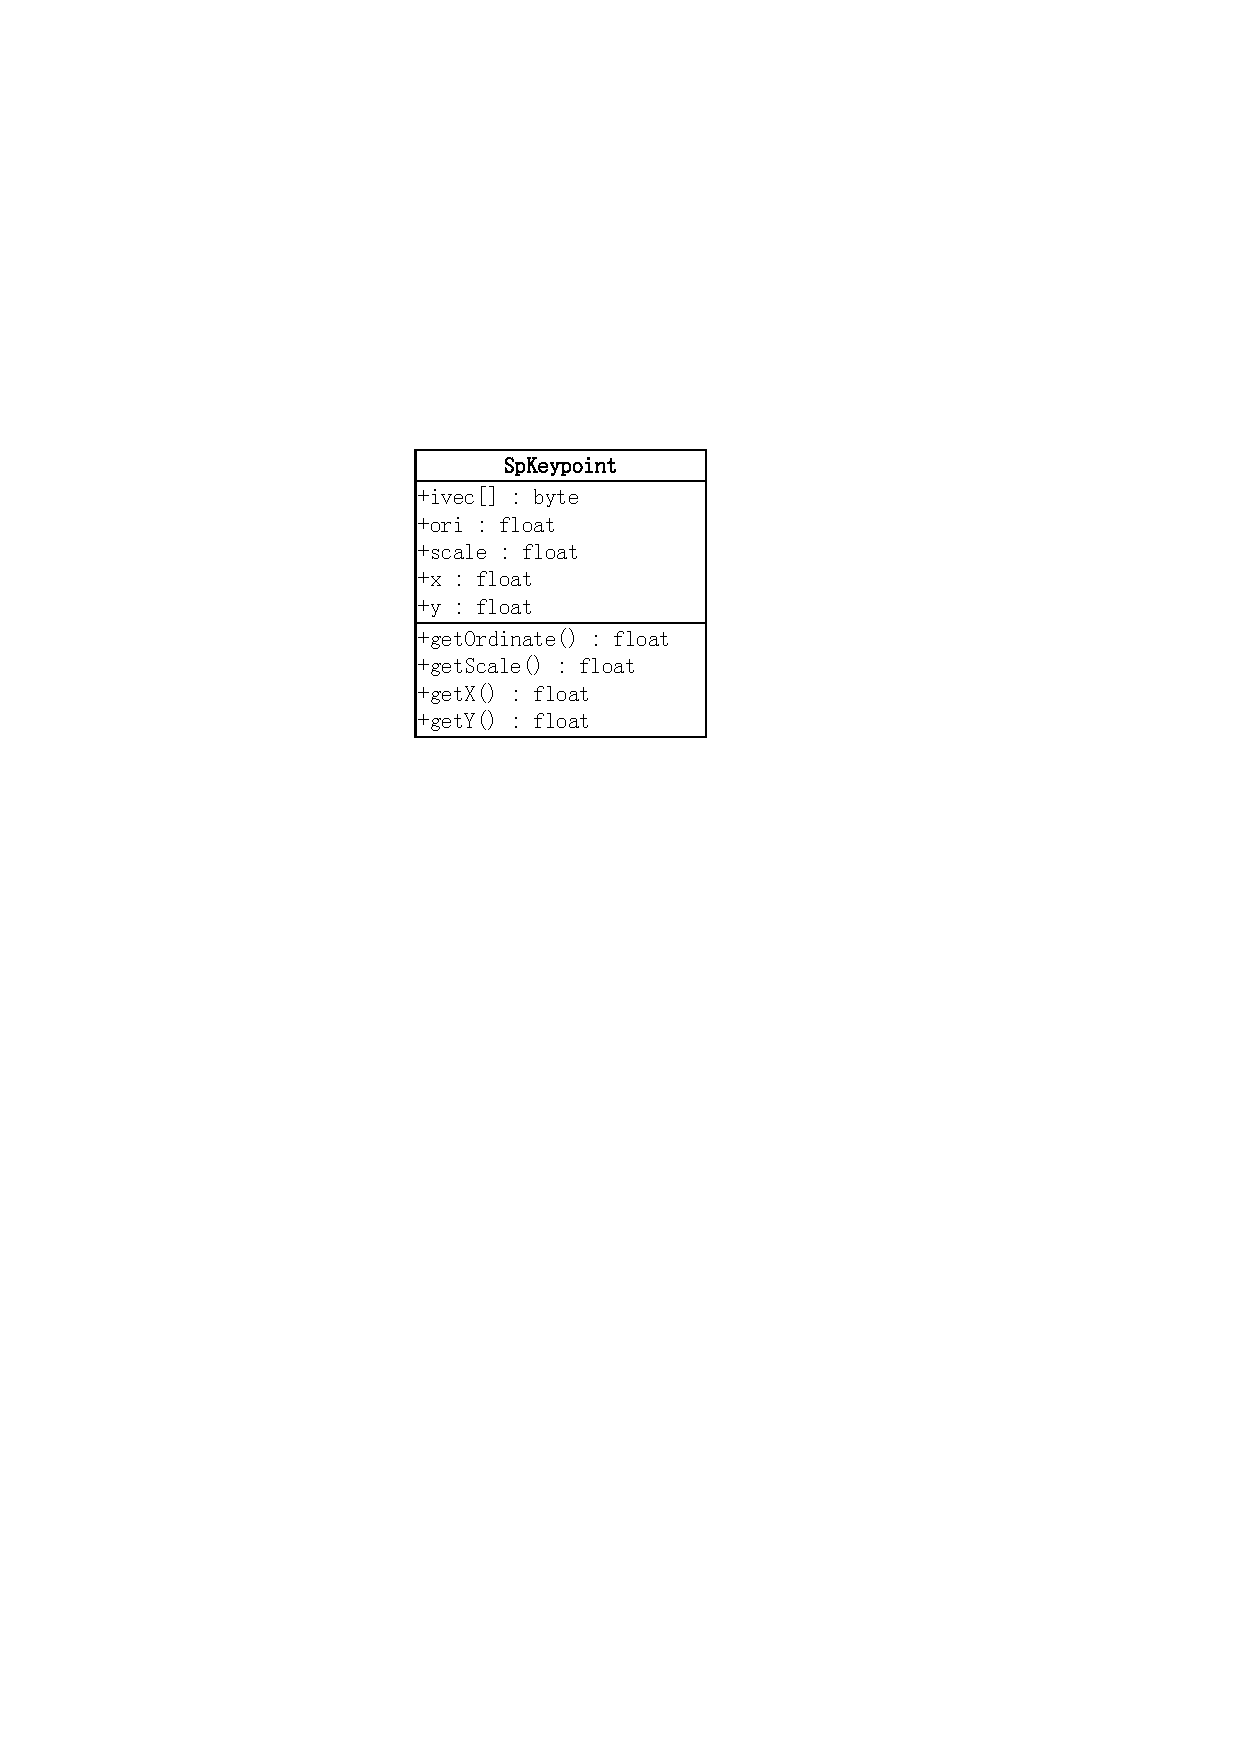
\includegraphics{spkeypoint}
\caption{SpKeypoint数据结构}
\label{fig:spkeypoint}
\end{figure}

其中x,y代表特征点在图片上的坐标,scale表示特征点的尺度大小,ori表示特征点的方向,ivec数组为特征点的一维描述向量,长度为128。

SpMemoryLocalFeatureList数据结构保存sift算法检测一张图片的所有特征点集,因此SpMemoryLocalFeatureList具有集合特性,本文设计时,让该类继承ArrayList,图\ref{fig:spmemflist}为SpMemoryLocalFeatureList的UML视图。
\begin{figure}[htp]
\centering
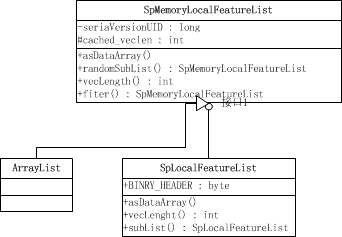
\includegraphics{spmemflist}
\caption{数据结构}
\label{fig:spmemflist}
\end{figure}

\subsection{spark-sift算法}
在这小节中将spark下怎样使用sift算法进行大规模图像库特征提取工作。主要的思想是利用上一小节介绍的spark-imagelib来实现整个sift算法,sift 算法在第二章原理分析中已经详细的分析过了,在此不再详述,然后利用spark的map-reduce框架,在map函数中调用已经实现好的sift算法,在提取结束后,将特征向量保存到HDFS中,完成整个特征提取的工作。spark-sift算法如图\ref{fig:alg_sparksift}所示:
\begin{figure}[htp]
\centering
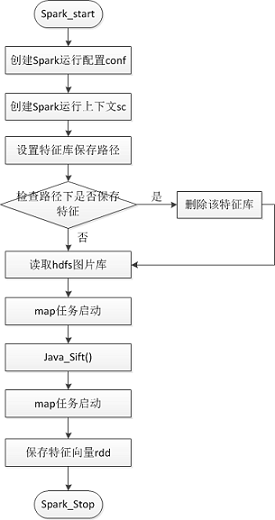
\includegraphics{alg_sparksift}
\caption{spark-sift算法流程}
\label{fig:alg_sparksift}
\end{figure}

spark-sift算法的关键伪代码如下:
\begin{lstlisting}[language=Java]
val conf = new SparkConf()//创建spark configure
conf.set()//设置configure
val sc = new SparkContext(conf)//创建spark 运行上下文

rm_hdfs(hdfs_name,kpslibdir+dataset)//删除原有的特征库

//并行执行图片特征提取任务
val fn_rdd = sc.sequenceFile(imageSEQ_path,task_size.toInt).map({
var datainput = new ByteArrayInputStream(fcontext.getBytes)

var img = SpImageUtilities.readF(datainput)
if(img != null){
    var engine = new SpDoGSIFTEngine()//进行sift 特征提取
    var kps = engine.findFeatures(img)

    val baos = new ByteArrayOutputStream()
    IOUitls.writeBinary(baos,kps)
    (new Text(fname.toString), new BytesWritable(baos.toByteArray))//以key-value形式返回提取的特征点,key为图片名,value为特征点集
}
})
\end{lstlisting}

通过上面这段代码,每张图片将被划分到不同的分区中,在每个分区中,执行特征提取任务,然后将得到的特征点以key-value的形式分布式保存到HDFS 中,其中key为图片的文件名,value为特征点集的字节流。
\subsection{序列化模块}
因为互联网上图片的体积一般都是1M以下,HDFS以Block形式进行存储,Block的大小是128M,因此这些文件对于HDFS来说都是小文件,众多的小文件存在时,就会造成频繁的磁盘IO,从而导致读写的性能降低。其实,这种场景在我们生活中也有体会,从U盘拷贝一个2G的文件和拷贝一个由很多小文件组成的2G文件夹,速度是相差很大的。

基于上述情况,本文在整个系统中加入了图片序列化模块,通过该模块将图片转化为key-value记录的形式,然后将众多的记录合并并且序列化保存到HDFS中,后续的处理都是在该序列化后的记录上进行,从而提升HDFS读写效率。本文会在第四章的性能优化中对序列化优化方案进行详细分析,在这里,主要介绍代码框架设计。序列化模块流程框架如图所示\ref{fig:alg_sequence}。
\begin{figure}[htp]
\centering
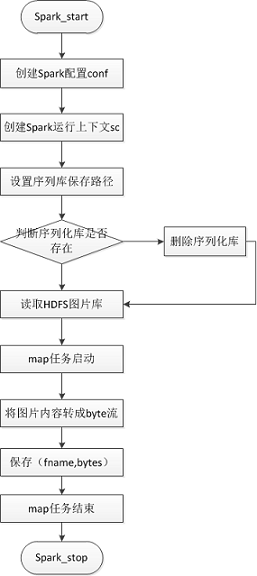
\includegraphics{alg_sequence}
\caption{序列化模块流程框架图}
\label{fig:alg_sequence}
\end{figure}

序列化模块关键伪代码如下:
\begin{lstlisting}[language=Java]
val conf = new SparkConf()//创建spark configure
conf.set()//设置configure
val sc = new SparkContext(conf)//创建spark 运行上下文

rm_hdfs(hdfs_name,path)//删除原有的序列库

//并行执行图片特征提取任务
val fn_rdd = sc.binaryFiles(initImgs_path,task_size.toInt).map(f =>{
val fname = new Text(f._1.substring(prefix_path_hdfs))//构造记录的key值

val bytes = f._2.toArray()
val fcontext = new BytesWritable(bytes)//将图片的内容转化成byte字节流

(fname,fcontext)//以序列化方式保存图片到hdfs
}).saveAsHadoopFile(path)
\end{lstlisting}

通过上面这段序列化预处理代码,每张图片将划分到不同的分区,在不同的分区中执行图片转成单条记录的形式的任务,最后记录以key-value的形式保存到hdfs中。
\subsection{存储模块}
在存储层设计,本文采用HDFS当作系统的存储层,将图像库,图像序列化库,图像特征集,错误信息均保存到HDFS中。因为面对着大规模数据时,单机存储的方案基本是不太现实的,所以本文采用了分布式的存储方案。HDFS是Hadoop下的产物,但是它和Spark的交互也十分方便。spark下提供有丰富的HDFS 操作API,通过这些API,基本上能满足开发者的需求。本文设计主要用到了HDFS的以下接口:
\begin{table}[h] %开始一个表格environment,表格的位置是h,here。
\caption{Spark-SIFT系统涉及的HDFS API} %显示表格的标题
\centering
\label{tab:HDFS_API}
\begin{tabular}{p{3cm}|p{8cm}} %设置了每一列的宽度,强制转换。
\hline
\hline
函数名  &  功能 \\ %用&来分隔单元格的内容 \\表示进入下一行
\hline %画一个横线,下面的就都是一样了,这里一共有4行内容
sequenceFile   & 读取hdfs序列化后的图片\\
\hline
binaryFiles   & 读取hdfs图片库图片\\
\hline
saveAsHadoopFile  & 将图片或者是特征点集以序列化方式保存到hdfs\\
\hline
FileSystem.get & 获取hdfs文件的句柄\\
\hline
FileSystem.delete & 删除hdfs文件\\
\hline
\hline
\end{tabular}
\end{table}
\subsection{容错模块}
在大数据处理中,系统的容错是一个十分重要的功能,因为处理的数据量太大,处理的时间太长,因此处理过程中发生一些错误是十分常见的情况,比如有可能处理的数据中有几个非法的数据,在Spark-SIFT系统处理过程中,我们经常就会碰到图片集合中有几张非法格式的图片。但是系统不能因为这个非法格式的数据而处理被中断或者是崩溃,因此大数据系统中应该有一套自己的容错机制。在Spark-SIFT中,系统中有一个模块会对图片格式的合法性进行判断,找出所有非法格式的图片,然后将这些文件名连同路径写到HDFS中非法文件保存目录下,系统会定期读取该目录,进行非法格式图片的删除。

在Spark中如果应用运行的过程出现了运行时的异常,应用会直接退出。因此针对这种情况,在Spark-SIFT系统进行特征提取时,我们对特征提取应用的每一个stage都加入了过滤功能,将一些非法的结果过滤掉,只传送合法的结果到下一个stage,这样系统就不会因为发生异常而直接退出。具体实现时,本文是采用了Scala中的Try异常捕捉机制,当采用这种异常捕捉机制时,结果的返回一个重新封装的数据结构,该数据结构包含正确和异常的两个结果,换而言之,什么类型的结果都会返回,具体需要什么,我们可以根据条件进行过滤删选。图\ref{fig:try_stage}显示了Spark-SIFT系统在一个stage结束之后的容错处理操作。
\begin{figure}[htp]
\centering
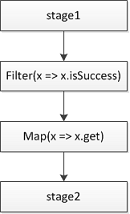
\includegraphics{try_stage}
\caption{stage和stage间的容错处理}
\label{fig:try_stage}
\end{figure}
%%需要做一些工作
\section{系统执行与验证}
在这小节中将会介绍整个Spark-SIFT大规模特征提取系统的编译,执行及正确性验证。
\subsection{spark-imageLib编译}
本文设计的图像基础库需要嵌入到spark系统中,因此需要和spark的源码一块编译,然后在spark应用开发中,以依赖的形式导入spark-imageLib库支持。本文使用的spark版本是2.0.0,其源代码可以在spark 官网或者是github网站下载。spark源码是一个maven工程,maven是一个高级的项目管理工具,可以管理项目中的所有依赖及其他配置。下面简要的介绍一下创建spark-imageLib的步骤:
\begin{compactenum}
\item 在spark源码根目录下创建一个新的maven工程,工程的groupId为org.apache.spark,artifactId为spark-imageLib\textunderscore2.11;
\item 修改spark源码根目录下的pom.xml文件,在modules配置项中加入module值为imageLib的配置项;
\item 编译源代码,编译命令为mvn clean install,该命令会重新编译spark源码,生成新的spark安装包,我们需要将新的spark安装包安装在集群上;
\end{compactenum}
\subsection{特征提取应用程序提交}
在spark特征提取应用程序中引用spark-imageLib库依赖,编写特征提取程序,编译生成分布式特征提取应用jar包,然后该jar包提交到spark运行集群上。提交命令如下:
\begin{code}
spark-submit
\\--class cn.zxm.scala.sparkImageDeal.ImagesFeatureEx
\\--master spark://hadoop0:7077
spark-SIFT-1.0.SNAPSHOT.jar
\end{code}
\subsection{正确性验证}
以280M的图片数据集为例子,该数据集共有1833张图片,简单展示一下从Spark-SIFT系统的特征提取功能,运行提取作业结果如图\ref{fig:find_finish} 所示。我们从该数据集中随机抽取了4张图片,分别是ILSVRC2012\textunderscore val\textunderscore00021292.JPEG,ILSVRC2012\textunderscore val\textunderscore00021324.JPEG,ILSVRC2012\textunderscore val\textunderscore00021353.JPEG 及ILSVRC2012\textunderscore\\val\textunderscore00021358.JPEG,使用这四张图片去查询匹配以验证提取的特征点的正确性,匹配程序中的匹配条件为匹配特征点数必须大于查询图片特征点的1/2,并且不能超过查询特征点总数。四张图片的匹配结果分别如图\ref{fig:00021292_match},图\ref{fig:00021324_match},图\ref{fig:00021324_match},图\ref{fig:00021358_match}所示,其中第一张图片查询特征点总数为362,匹配查询结果为一张,错误率为0\%,匹配点数为296;第二张图片查询特征点总数为1030,匹配查询结果为一张,错误率为0\%,匹配点数为898;第三张图片查询特征点总数为400,匹配查询结果为一张,错误率为0\%,匹配点数为317;第四张查询特征点数为351,匹配查询结果为5张,错误率为0.27\%,和原图匹配的特征点数为318,在所有的匹配图片中是最高的。
\begin{figure}[htp]
\centering
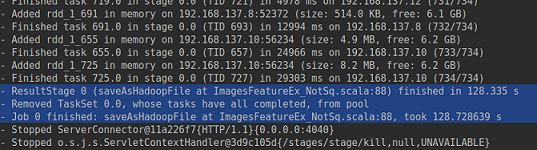
\includegraphics{find_finish}
\caption{提取作业结果}
\label{fig:find_finish}
\end{figure}

\begin{figure}[htp]
\centering
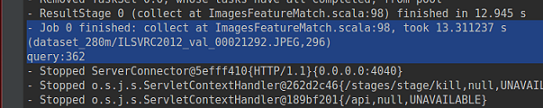
\includegraphics{00021292_match}
\caption{00021292图片匹配结果}
\label{fig:00021292_match}
\end{figure}

\begin{figure}[htp]
\centering
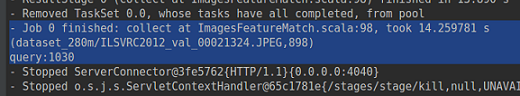
\includegraphics{00021324_match}
\caption{00021324图片匹配结果}
\label{fig:00021324_match}
\end{figure}

\begin{figure}[htp]
\centering
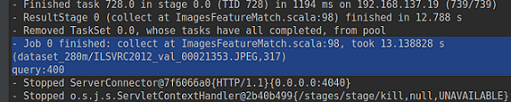
\includegraphics{00021353_match}
\caption{00021353图片匹配结果}
\label{fig:00021353_match}
\end{figure}

\begin{figure}[htp]
\centering
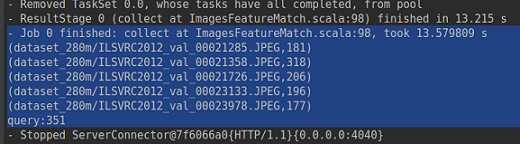
\includegraphics{00021358_match}
\caption{00021358图片匹配结果}
\label{fig:00021358_match}
\end{figure}

\section{本章小结}
本章主要介绍了大规模图像库特征提取系统Spark-SIFT的设计和实现,首先介绍了系统的主要框架,从软件架构的角度分析了系统的每一个模块的设计和实现,分别介绍了spark-imageLib,spark-sift算法,序列化模块,存储模块以及容错模块。最后展示了特征提取系统的编译执行及提取结果。

\chapter{Spark-SIFT系统的三种性能优化方案}
在上一章节中,本文介绍了整个大规模特征提取系统Spark-SIFT的设计和实现,本章节主要针对Spark-SIFT进行性能优化。第一,针对Spark-SIFT系统加载大量小图片时,频繁的磁盘IO,读写开销较大问题作出了优化,在该问题的优化上,本文设计了一种新的数据结构来描述图片,以Key-Value的方式表示一张图片,将图片转成单条记录的形式,然后将众多的记录合并并且序列化保存供后续操作使用,以提高读写效率;第二,由于Spark的任务划分及分配机制,导致Spark-SIFT系统在处理图片大小差异很大的数据集,会出现负载不均衡的现象,本文提出了分割式特征提取算法以解决处理过程中出现的负载不均衡问题;第三,因为分割式特征提取算法会引用shuffle操作,当处理的图片量很大时,会严重影响系统的性能,因此本文在分割式特征提取算法的基础上改进,提出了shuffle-efficient的特征提取算法,以解决shuffle操作带来的性能问题。

\section{key-value的图片描述数据结构}
因为图片和图片间是分立的,整个数据集是一个个分立的文件组成,spark在加载的时候也只能是一个个加载,如果每个文件很小,文件的数量有多,这情况下读写的效率是很低的。那么怎样才能提高加载时候的性能呢?在spark下处理文本信息会比较多,在处理文本信息时,spark是把一整个文本文件加载进来,然后每一行就是一个基本的并行单元,所以能不能把一张图片看成文本文件中的一行记录,然后很多行记录组成一个大文本,就相当很多个图片合并在一个大文件中,那么一次性就可以加载很多图片。

在spark在处理文本文件方式的启发下,我们采用了Key-Value的方式来描述一张图片,Key就是图片的文件名,Value就是图片内容的字节流,通过这种方式,就可以用一条记录的形式描述了一张图片,然后将这些记录序列化保存到指定的hdfs目录下,在序列化方式上,Spark-SIFT选用了Hadoop的原生序列化方式,而没有采用Java序列化。这是因为Java序列化后产生的内容容量太大,分布式环境中传输时会十分占用带宽,而hadoop序列化产生的内容十分简洁,容量更小,这有助于减少分布式处理时的数据传输量。通过这种将图片转换成记录的形式,Spark在读取该目录时,就可以一次性将目录下的记录加载进来,从能提供了读写的效率。图\ref{fig:kv_image}显示了整个设计的框架。
\begin{figure}[htp]
\centering
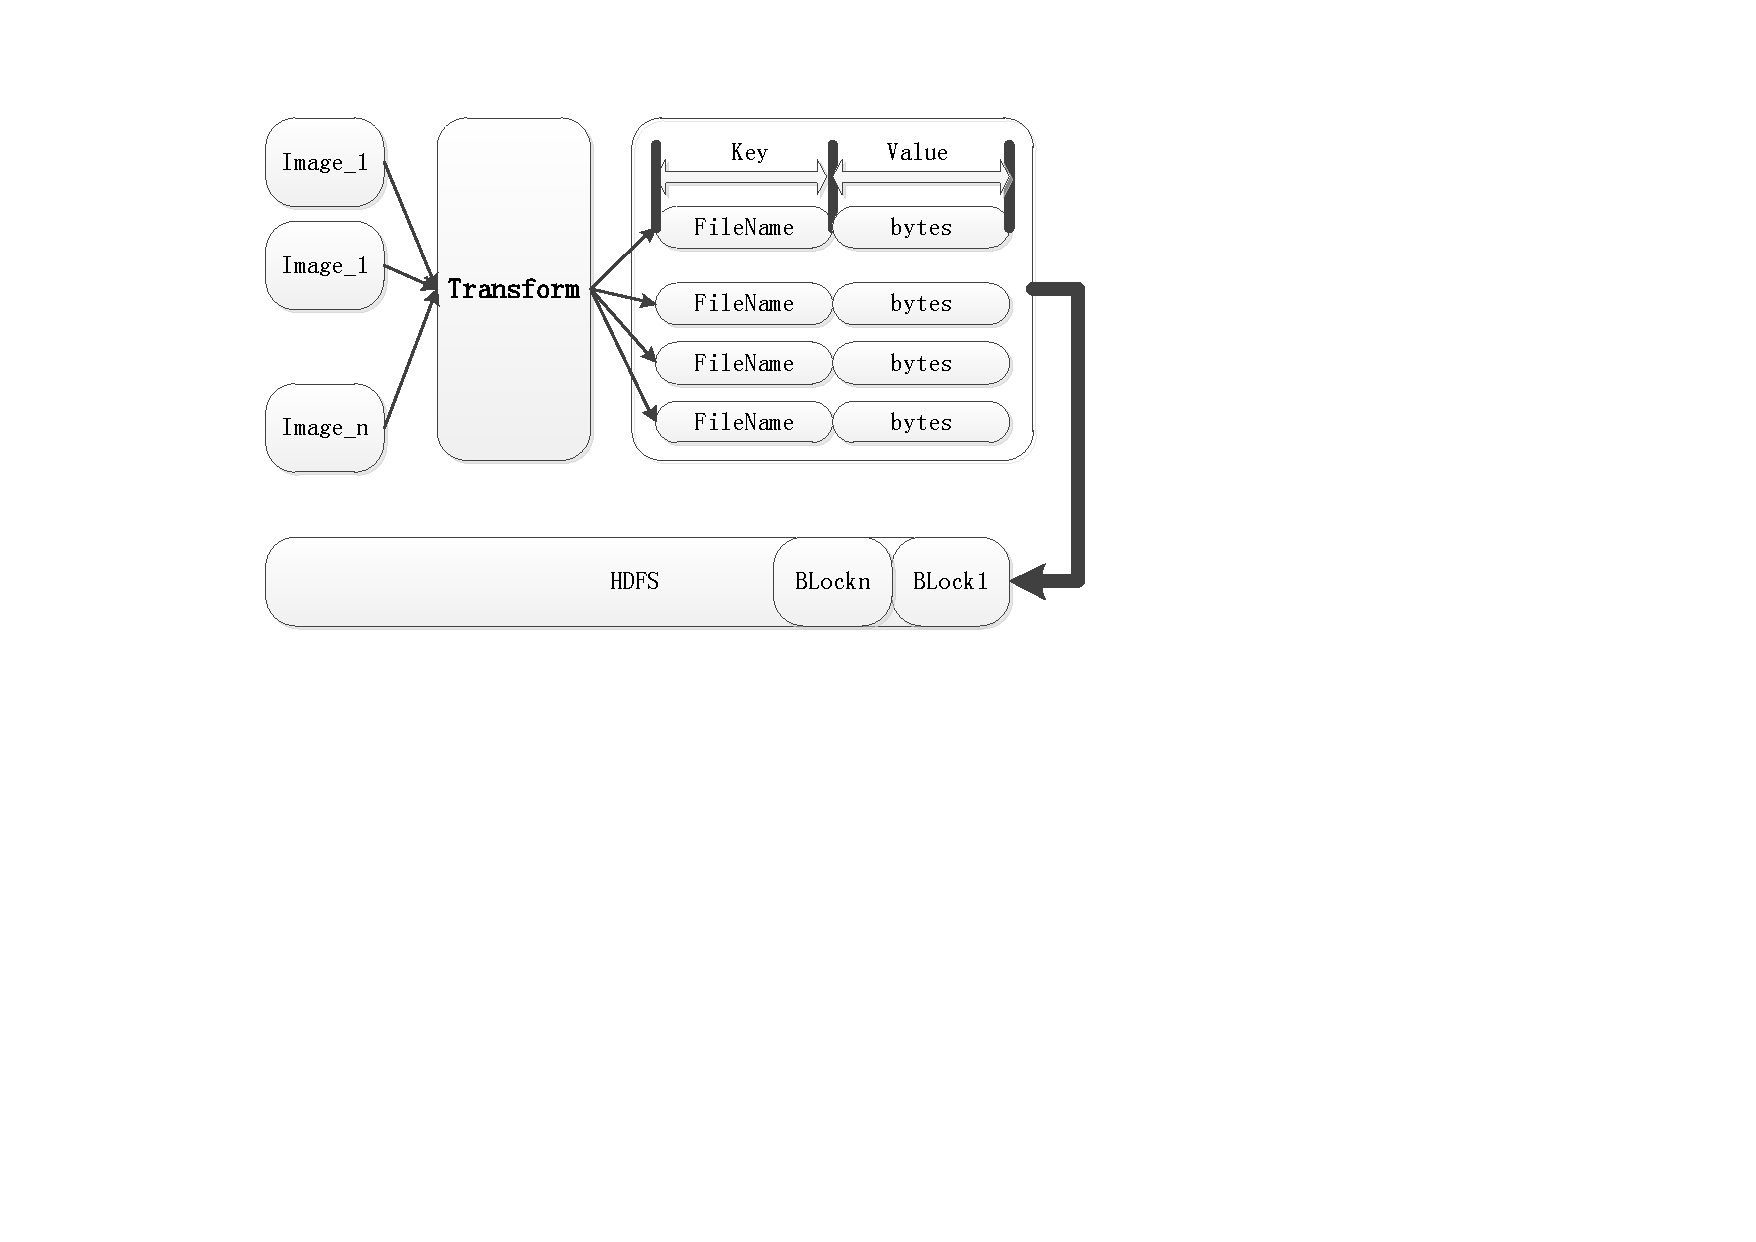
\includegraphics{kv_image}
\caption{key-value描述图片方式}
\label{fig:kv_image}
\end{figure}

具体的实验数据将会在第五章中给出,在此先不进行数据的分析。
\section{分割式图片特征提取算法}
Spark-SIFT在对某些数据集进行特征提取时会出现严重的负载不均衡现象。以提取200MB图片集合的特征为例,集合中图片的大小为2MB或4MB,但其处理时间有时会比处理一个1GB 的图片集合(图片大小在100到200KB之间)还要长。观察Spark的Executors监控页面我们发现,200MB图片集处理时间较长往往是因为某个Executor的执行速度特别慢,而此时其他Executors都已经完成了分配的任务,处于空闲状态。

有两个原因引发了Spark-SIFT系统在处理图片差异较大数据集时出现的负载不平衡现象。首先与SIFT算法自身的特点有关,SIFT算法的时间复杂度和图片大小相关,为$O(N^5)$,并且SIFT算法的空间复杂度也十分大,另外Spark本身也是很耗内存,这样就导致运行过程中很耗内存,当内存占用过高时,CPU的利用率无法上去,这样就导致运算速度十分慢;其次是Spark任务分配机制,Spark任务分配按照大小区分,划分时仅考虑了各个任务所处理的图片总容量,而忽略了任务中图片大小的因素。那么,如果图片的大小不一样,一个任务都是大图片,而另外一个是小图片,那么大图片的运行时间会更长,但是Spark分配机制认为只要两个任务是size一样,那么两个任务运行时间基本一样。同时Spark分配到Executor 上的任务,在没有失败的情况下,是不会回收的,尽管有其他空闲的Executor,这样就会出现其他Executors都是空闲的,而只有一个Executor在运算的情况。

针对上面的问题,我们采用分割图片的方式,使图片集中各图片的大小尽可能相同,以适应Spark的任务分配和负载均衡策略,使各个任务的运行时间基本相同。图片分割的具体工作原理如图\ref{fig:segmentation}所示:
\begin{figure}[htp]
\centering
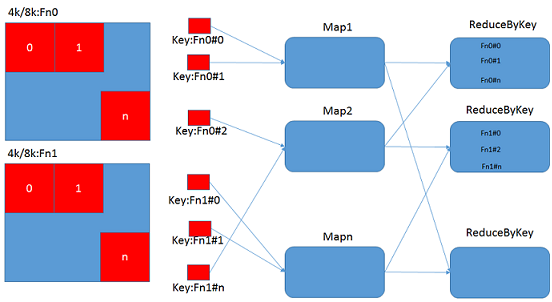
\includegraphics{segmentation}
\caption{分割式特征提取算法}
\label{fig:segmentation}
\end{figure}

本文将分割后得到的图片大小称为分割大小,它会影响特征提取的速度和结果的精度。理论上,分割后的图片越小,每张图片的处理速度越快,但是由于子图之间会产生边缘噪声,导致提取出的特征点存在较大的误差。通过实验,我们选择500×500作为基本分割大小,它既可以保证特征提取的速度足够快,又可以使得结果误差比较小,第五章将详细介绍测试结果和选择依据。

算法流程如图\ref{fig:alg_segmentation}所示,在map任务1,我们将一张图片按照设置的模板大小进行划分,划分为多个子块,每个子块由图片文件名加模块下标,模块的长,模块的宽以及模块的像素内容字节数组四个元素组成。因为在map任务1结束后,一张图片的子块只是位于一个独立的数组中,数组和数组间是分立的,这样并行操作只能在单个数组里面进行,这种情况并行化程度是不高的,因此在map任务1结束后,我们又启用了一个flatMap算子,通过flatMap操作,我们将数组扁平化,将每个数组的元素抽取出来,组成一个大的数组,使得并行化操作在所有图片的子块中执行,这样就可以大大提高并行化程度。当图片子块被扁平化之后,我们又重构了子块的表示方式,在map 任务1中,子块的表示方式是(fname,row,col,bytes),在map任务2 中,以(fname,(row,col,bytes))的方式表示一个子块,这样子块就可以表示为key-value的形式了,这种表示方式也为后面处理完子块后收集同一张图片的子块提供了方便;在map任务3中,进行子块图片的特征提取工作,在这个任务中,我们还进行key的重构工作,因为之前子块的key是带有下标的,但是在特征提取完之后就不需要带有下标了,因此我们将子块图片的下标去掉,那么同一张图片的子块的key就是一样的,最后提取的出来的特征点集以(fnkey,kpslist.tolist)的形式表示,其中fnkey就是子块图片的所属图片的文件名,kpslist就是子块图片提取的特征点集合,kpslist.tolist表示将其转化成list的形式;在map 任务3结束后,我们启动了一个reduceByKey 的任务,在该任务中,我们按照key进行value合并,通过这个操作,同一张图片的划分为不同子块提取的特征点集就会收集到一个数组中,数组的每一个元素对应子块提取的特征点集;在最后的一个任务map任务4中,我们将提取的特征点集进行序列化,最后保存到HDFS中。
\begin{figure}[htp]
\centering
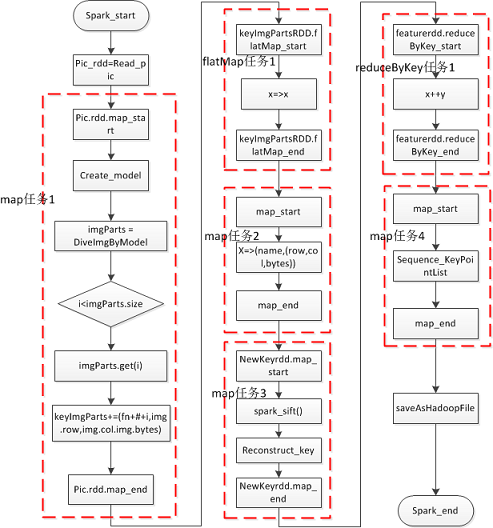
\includegraphics{alg_segmentation}
\caption{分割式特征提取算法流程图}
\label{fig:alg_segmentation}
\end{figure}

子块划分算法如下所示:
\begin{algorithm}[htbp]
  \caption{子块划分算法}
  \label{algDiveModel}
  输入:原始图片像素数组orgin,划分模板modelImg\\
  输出:子块数组imgParts
  \begin{algorithmic}[1]
    \STATE $rowParts\leftarrow imgrow/modelImg.row$
    \STATE $colParts\leftarrow imgcol/modelImg.col$
    \FOR{$i=0$ to $rowParts$}
    \IF{$i==rowParts-1$}
        \STATE $rowOffset\leftarrow row + imgrow\%modelImg.row-1$
    \ELSE
        \STATE $rowOffset\leftarrow row - 1$
    \ENDIF
    \FOR{$j=0$ to $colParts$}
    \IF{$j==colParts-1$}
        \STATE $colOffset\leftarrow col + imgcol\%modelImg.col-1$
    \ELSE
        \STATE $colOffset\leftarrow col - 1$
    \ENDIF
    \STATE $img\leftarrow getOnePart$
    \STATE imgParts.add(img)
    \ENDFOR
    \ENDFOR
    \STATE Return imgParts
  \end{algorithmic}
\end{algorithm}

算法是利用模板进行逐行扫描思想,1,2两步获取图片被划分的块数,第3步进入一个嵌套循环,分别是按rowParts和colParts遍历,根据rowOffset和colOffset依次得到相应的子块,获取步骤为第15步,将每次获取到的子块添加到imgParts数组中,函数结束后返回imgParts数组。 因为图片大小和模板大小不是一个整倍数的关系,所以在嵌套遍历中加入了最后一次的特殊处理,直接赋值rowOffset 和colOffset,即第5 步和第7 步。获取子块函数getOnePart关键伪代码如下所示:
\begin{lstlisting}[language=Java]
public static SequenceImage GetOnePart(byte [][]pixel, int rowStart, int colStart, int roffset, int coffset){
    byte [][]tpixel = new byte[roffset+1][coffset+1];

    //根据行偏移和列偏移获取相应区域的像素块
    for (int i = 0; i <= roffset; i++) {
        for (int j = 0; j <= coffset; j++) {
            tpixel[i][j] = pixel[i+rowStart][j+colStart];
        }
    }

    SequenceImage partimg = new SequenceImage(roffset+1,coffset+1,tpixel);

    return partimg;//返回指定像素块
}
\end{lstlisting}

至此,分割式特征提取算法介绍完毕,在第五章中,我们会给出相应的实验数据分析。
\section{Shuffle-Efficient的特征提取算法}
在上一节中,本文介绍了分割式特征提取算法,在该算法中,我们将大图片划分为子块,目的是解决Spark-SIFT系统提取过程中出现的负载不均衡问题。虽然分割式解决了处理过程中负载不均衡问题,但是该算法也引入了Shuffle操作,Shuffle操作是spark处理中十分影响性能的一个操作,因此本小节中将会针对分割式提取算法中的Shuffle操作进行优化,以进一步提高Spark-SIFT系统的处理性能。
\subsection{Shuffle原理}
Spark在执行Map-Reduce操作时,需要将处理的数据集分发到各个节点上,在数据被处理完后,再从各个节点上回收结果,这就是一个具有Shuffle操作的过程。Shuffle操作存在大量的磁盘IO和网络传输,十分损耗性能。spark中存在两种Shuffle机制,分别是Hash Based Shuffle机制和Sort Based Shuffle机制。Hash Based Shuffle,正如名字所示,该Shuffle机制是跟Hash值相关的,这个Hash值指的是key的Hash值,Spark会根据key的Hash值算出对应的分区,这个分区其实就是下游的一个任务,然后将上游任务的结果单独的写到一个文件中,下游的任务拉取相应的结果文件,继续任务的执行,整个过程如图\ref{fig:hash_shuffle}所示。
\begin{figure}[htp]
\centering
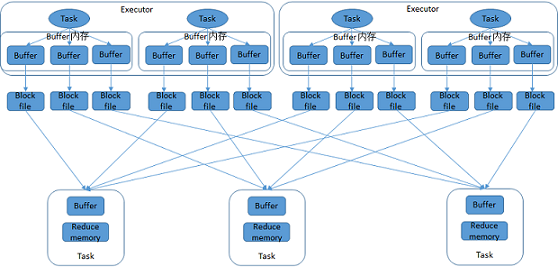
\includegraphics{hash_shuffle}
\caption{hash based shuffle机制}
\label{fig:hash_shuffle}
\end{figure}

从Hash Based Shuffle的运行过程就可以看出,每个上游的任务都需要给下游的任务创建一个文件,过程产生文件的总数为:tasks(上游)*tasks(下游),在图\ref{fig:hash_shuffle} 中就创建了4*3个过程文件,如果上游和下游的任务数很多,那么就会有大量的中间文件被创建,而每打开一个文件都会占用内存,这将消耗大量的内存,很容易就造成内存溢出;另外读写大量的文件就会存在大量的磁盘IO操作,这也是十分损耗性能的,并且如果同一个key的结果文件散落在不同的机器的分区上,又会存在网络传输的开销。

针对Hash Based Shuffle产生大量中间文件的问题,Spark中又出现了一个Sort Based Shuffle机制,在该机制下,每个上游的任务会把结果只写到一个文件中,然后生成一个index,下游的任务根据index的信息,到对应的文件上读取上游结果信息。通过这样方式,就可以大大的减少中间文件的数量,如图\ref{fig:sort_shuffle}所示,该方式下,过程文件仅为4个。
\begin{figure}[htp]
\centering
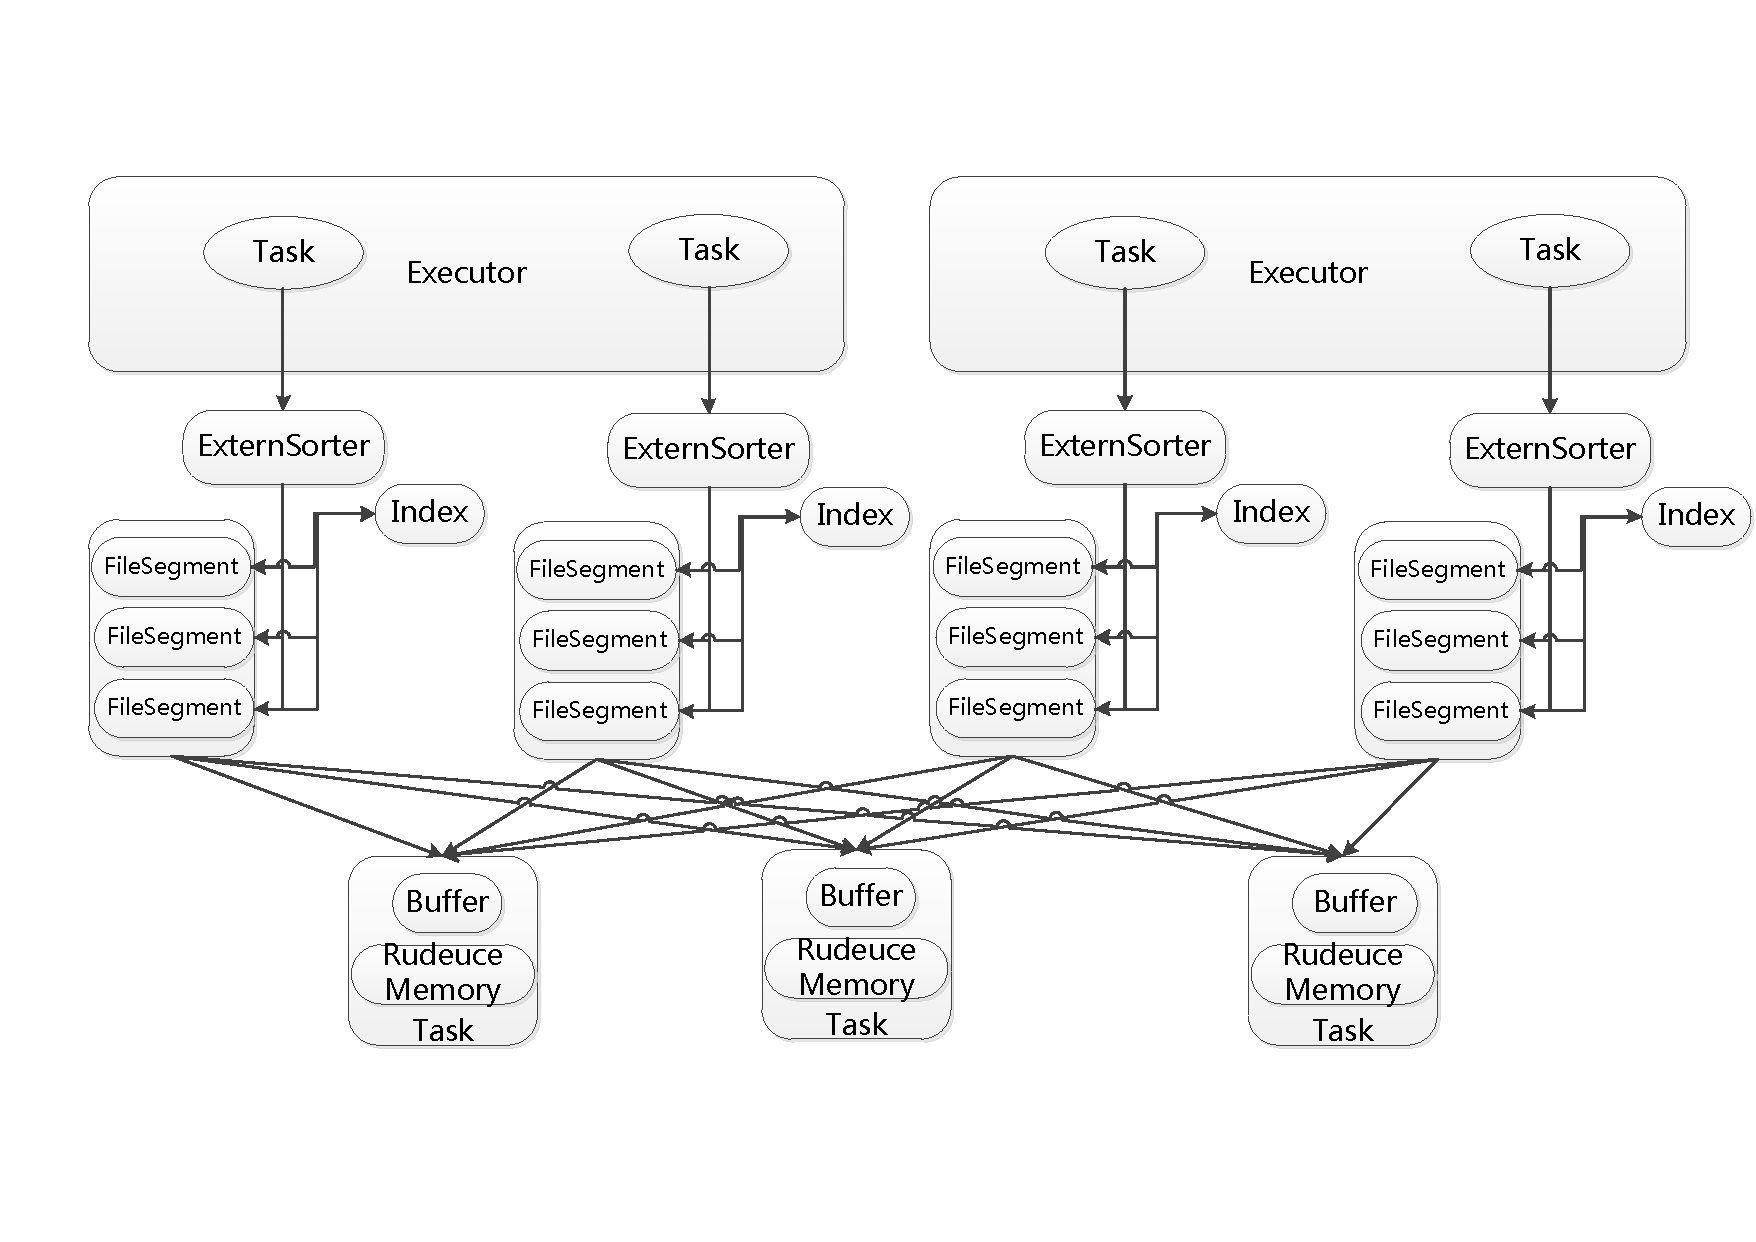
\includegraphics{sort_shuffle}
\caption{sort based shuffle机制}
\label{fig:sort_shuffle}
\end{figure}

\subsection{高效的分区划分}
如图所示\ref{fig:seg_shuffle}在分割式算法中是存在两个Shuffle过程的,分别是将图片的子块分配到不同的分区上以及从不同的分区中收集子块特征点集,因为每张图片的子块在被收集之前,它们的key是不相等的,根据之前分割式算法分析中,它们是用图片的文件名加上子块位于图片的下标组成的。如果按照Spark的默认分区策略,Spark会按照Key的哈希值进行分区,那么同一张图片的子块就有可能会被分配到不同的分区上,也就有可能位于不同的机器上。所以当出现这样情况时,在收集同一张图片的子块时,就需要跨分区和跨机器收集,这显然会影响性能。因此本文提出了一种高效的分区策略,我们对子块进行分区时没有使用Spark的默认分区策略,而是截取了子块key字符串的`\#`之前的字符串,然后算这个字符串的hash值,根据该hash值对总分区数的求余值进行分区。因为同一张图片的子块它们的key字符串中`\#`字符之前的字符串是一样的,那么算出来的hash值也是一样的,所以它们的分区号也是一样的。通过这种分区方式,就可以使得同一张图片的不同子块落在同一分区上,减少了无谓的跨分区收集的网络传输开销。分区划分算法如下所示:
\begin{algorithm}[htbp]
  \caption{高效分区策略}
  \label{algDiveModel}
  输入:子块key字符串\\
  输出:子块分区号
  \begin{algorithmic}[1]
    \STATE $newKey\leftarrow key.split("\#")$
    \STATE $code\leftarrow newKey.hashCode\%numPartitions$
    \IF{$code<0$}
        \STATE $code\leftarrow code + numPartitions$
    \ENDIF
    \STATE Return code
  \end{algorithmic}
\end{algorithm}

\begin{figure}[htp]
\centering
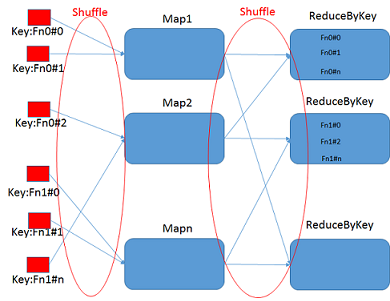
\includegraphics{seg_shuffle}
\caption{分割式算法的Shuffle操作}
\label{fig:seg_shuffle}
\end{figure}

\section{本章小结}
本章主要介绍了针对Spark-SIFT系统的三种优化策略。首先是针对大量小文件在spark中加载低效问题,本文设计了一种用key-vaule表示图片的数据结构,将一张图片转化成一条记录,然后将多条记录合并保存,从而提高了Spark加载处理图片的效率;其次,本文针对Spark-SIFT 系统在处理图片大小差异较大的数据集时出现的负载不均衡问题,本文提出了分割式特征提取算法,将大图片划分为子块,解决了Spark-SIFT系统的负载不均衡问题同时也提高了系统的并行度;最后,本文针对分割式特征提取算法中引入的Shuffle开销,提出了Shuffle-Efficient的特征提取算法,使用了高效的分区策略,降低了Shuffle的网络开销。

\chapter{Spark-SIFT性能测试和分析}
\section{实验环境}
本文构建了一个包含7台PC机的PC集群作为Spark-SIFT 系统的性能测试和分析实验平台,实验平台集群的主要配置参数如下:
\begin{compactenum}
\item 集群总体配置7台PC,其中1台master,6台worker;Spark的版本为2.0.0,集群的管理模式采用Spark原生的standalone模式。
\item Master节点配置为:处理器AMD APU,内存为16GB,硬盘为1TB,操作系统为Ubuntu 14.04;
\item Slave节点配置为:处理器Intel,内存12GB,硬盘为1TB,操作系统为Ubuntu 14.04;
\end{compactenum}

因为实验中,我们还选取了GPU作为对比试验,GPU的配置为NVIDIA GTX760,CUDA 4.0。

在测试数据集上,在测试Key-Value图片描述性能时,我们从ImageNet 2012\upcite{Imagenet}中随机选择了8个不同规模的图片集作为测试输入,分别是500KB (8),70 MB(530),140 MB(1003),280 MB(1833),1 GB(8719),2 GB(15024),4 GB (28721)和11 GB(78492),圆括号中为图片文件的数量。在测试分割式图片特征提取算法及Shuffle-Efficent特征提取算法时,本文采用作者平时搜集到的高清图片作为测试数据集,这是图片大都是2M 以上,最大有4M多。
\section{实验结果与分析}
在实验设计上,本文首先分析Key-Value图片描述方式,分割式特征提取算法以及Shuffle-Efficient特征提取算法这三种优化策略的性能。最后本文将Spark-SIFT系统分别和SIFT的单机版本,GPU版本对比,分析性能的差异。
\subsection{key-value图片描述方式}
在key-value图片描述方式的性能分析上,本文和binaryFile以及objectFile两种方式进行对比,对比它们在加载不同的数据集大小图片所要耗费的时间,如图\ref{fig:data_loadPerformance}所示,测试时,采用的并行任务数是100个,当加载的图片数据较小时,三种加载方式并没有什么较大的差距,比如加载140M 时,Key-Value图片描述方式的加载时间为6S,binaryFile加载方式的加载时间为8S,objectFile加载方式的加载时间为8S。当加载的规模增大时,Key-Value方式的加载性能就提升的较为明显,在加载11G图片数据集时,Key-Value方式的加载时间为39S,binaryFile加载方式的加载时间为102S,objectFile加载方式的加载时间为234S,Key-Value图片描述方式的加载速度相对于binaryFile方式为2.6倍,相对于objectFile方式为6 倍。因此在加载众多小文件时,本文设计的Key-Value 图片描述方式大大的提高了加载的性能。

\begin{figure}[htp]
\centering
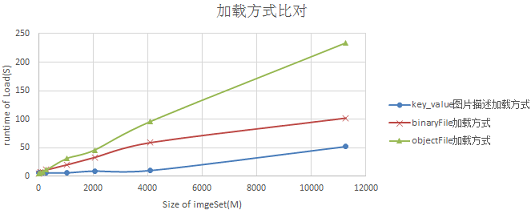
\includegraphics[width=148mm,height=84mm]{data_loadPerformance}
\caption{三种图片集合的加载性能比较}
\label{fig:data_loadPerformance}
\end{figure}
因为Key-Value方式是存在一个序列化预处理过程的,为了设计更加有说服力,本文也测试了序列化预处理时间占总处理时间的比例,同时如图\ref{fig:data_keyValue_ratio} 所示,随着图片集规模的增加,序列化时间占总处理时间的比例也在不断减小。当图片规模小于280MB 时,序列化时间占总处理时间的比例较高,超过了10\%;随着图片集的不断增大,序列化时间占总运行时间的比重会略微下降,对于11GB 的图片集合,序列化时间为300s,约占总处理时间的8\%。所以在处理大规模数据时,预处理并不会占用太多时间。
\begin{figure}[htp]
\centering
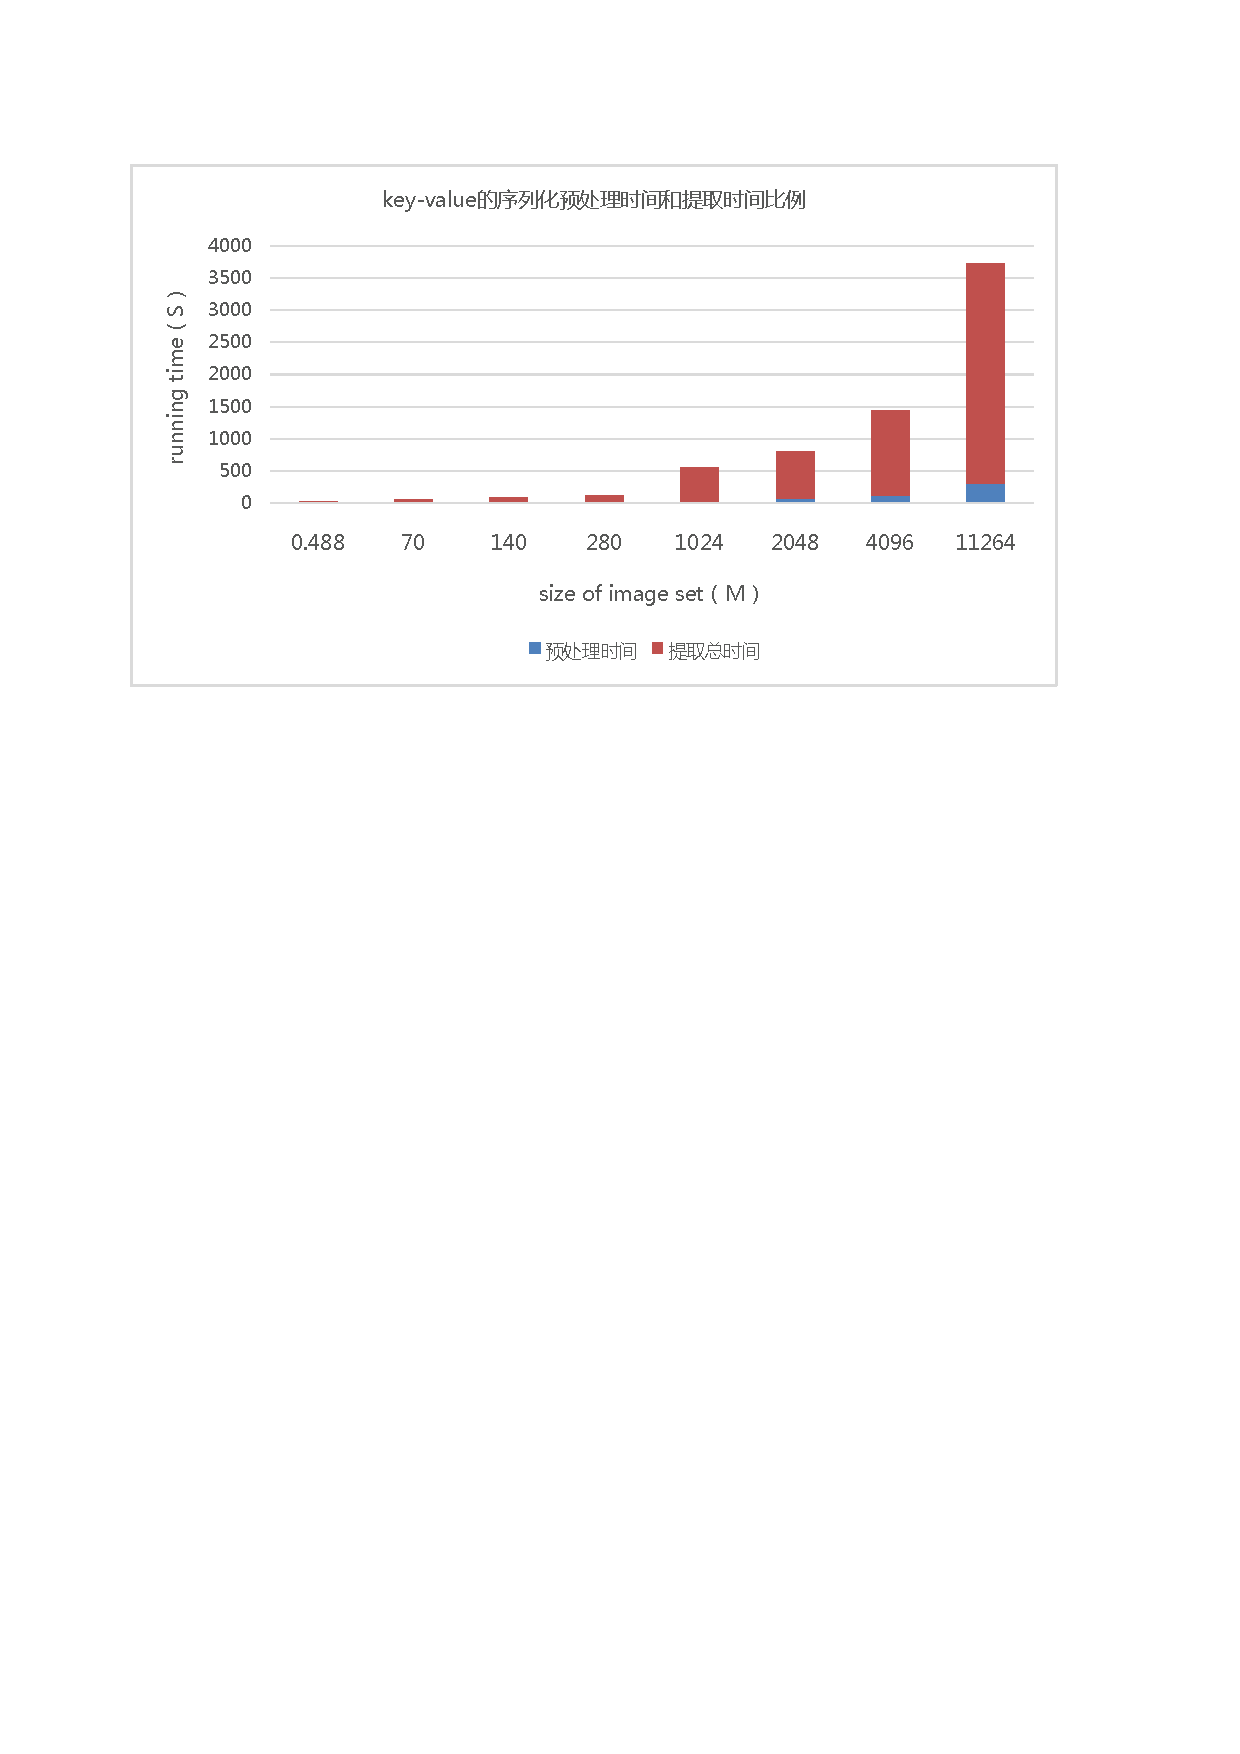
\includegraphics[width=148mm,height=84mm]{data_keyValue_ratio}
\caption{key-valuede的预处理时间和提取时间比例}
\label{fig:data_keyValue_ratio}
\end{figure}

\subsection{分割式特征提取算法}
在测试图片分割策略的优化效果时,我们采用了总容量为480MB的图片集合作为输入。集合中有280MB的``小`` 图片,其大小在100到200KB 之间,而其余200MB则是`` 大``图片,图片大小在2到4MB之间。当图片大小的差距增大时(例如KB与GB,或MB与GB),这种优化带来的性能提升将更加明显。图\ref{fig:data_seg_speed}描述了在不同的分割大小下,Spark-SIFT完成特征处理的时间。如图\ref{fig:data_seg_speed}所示,分割大小越小,提取的速度越快,例如在10×10的分割大小下,提取全部480MB图片特征的时间仅为210秒。但是如图\ref{fig:data_seg_accuracy}所示,分割大小越小,提取出的特征点的误差也越大,例如在10×10的分割大小下,误差率约为12\%。因此,综合提取速度和提取精确率两个因素,本文选取500×500作为分割大小。
\begin{figure}[htp]
\centering
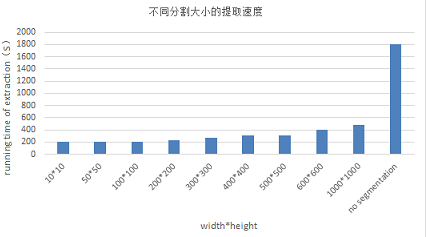
\includegraphics[width=148mm,height=84mm]{data_seg_speed}
\caption{不同分割大小的提取速度}
\label{fig:data_seg_speed}
\end{figure}

\begin{figure}[htp]
\centering
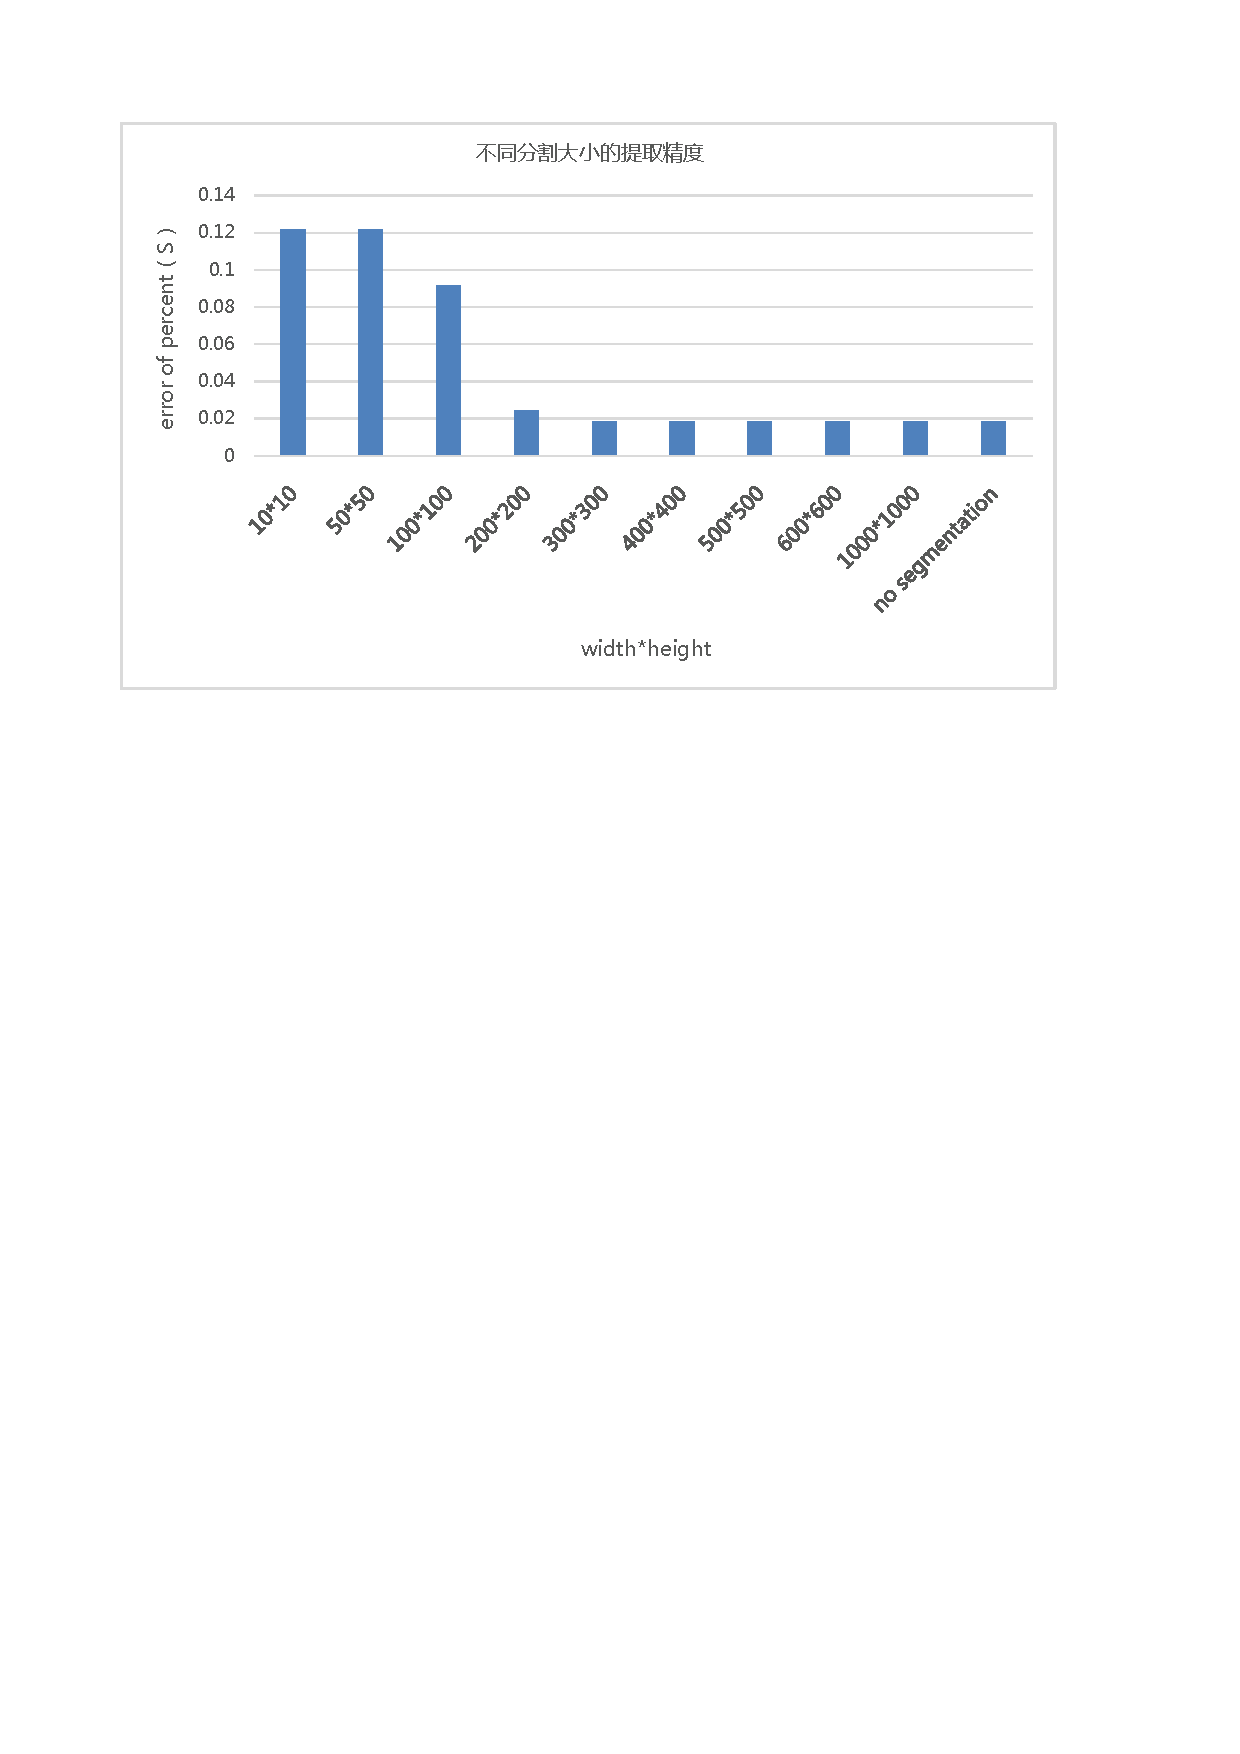
\includegraphics[width=148mm,height=84mm]{data_seg_accuracy}
\caption{不同分割大小的提取精度}
\label{fig:data_seg_accuracy}
\end{figure}

\subsection{Shuffle-Efficient特征提取算法}
在验证Shuffle-Efficient特征提取算法的有效性上,本文将采用高效分区策略的Shuffle-Efficient提取算法和采用Hash分区策略的分割式提取算法进行比较,在不同的测试图片数据集下对比它们在reduceByKey 步骤上所耗费的时间,以及Shuffle的数据量大小。如图\ref{fig:data_Partition}所示,本文对高效分区策略和Hash分区策略分别测试了3.2G及6.8G两组图片数据集。当数据集为3.2G时,采用高效分区策略的子块收集时间为169.087S,采用Hash分区策略的收集时间为199.742S,时间减少了大约30S,收集性能提高了约15\%,当测试规模增大到6.8G时,高效分区的收集时间为383.532S,Hash分区的收集时间为546.007S,收集性能提高了29.7\%,说明图片数据集越大时,高效的分区策略越能减少收集子块时产生网络开销。
\begin{figure}[htp]
\centering
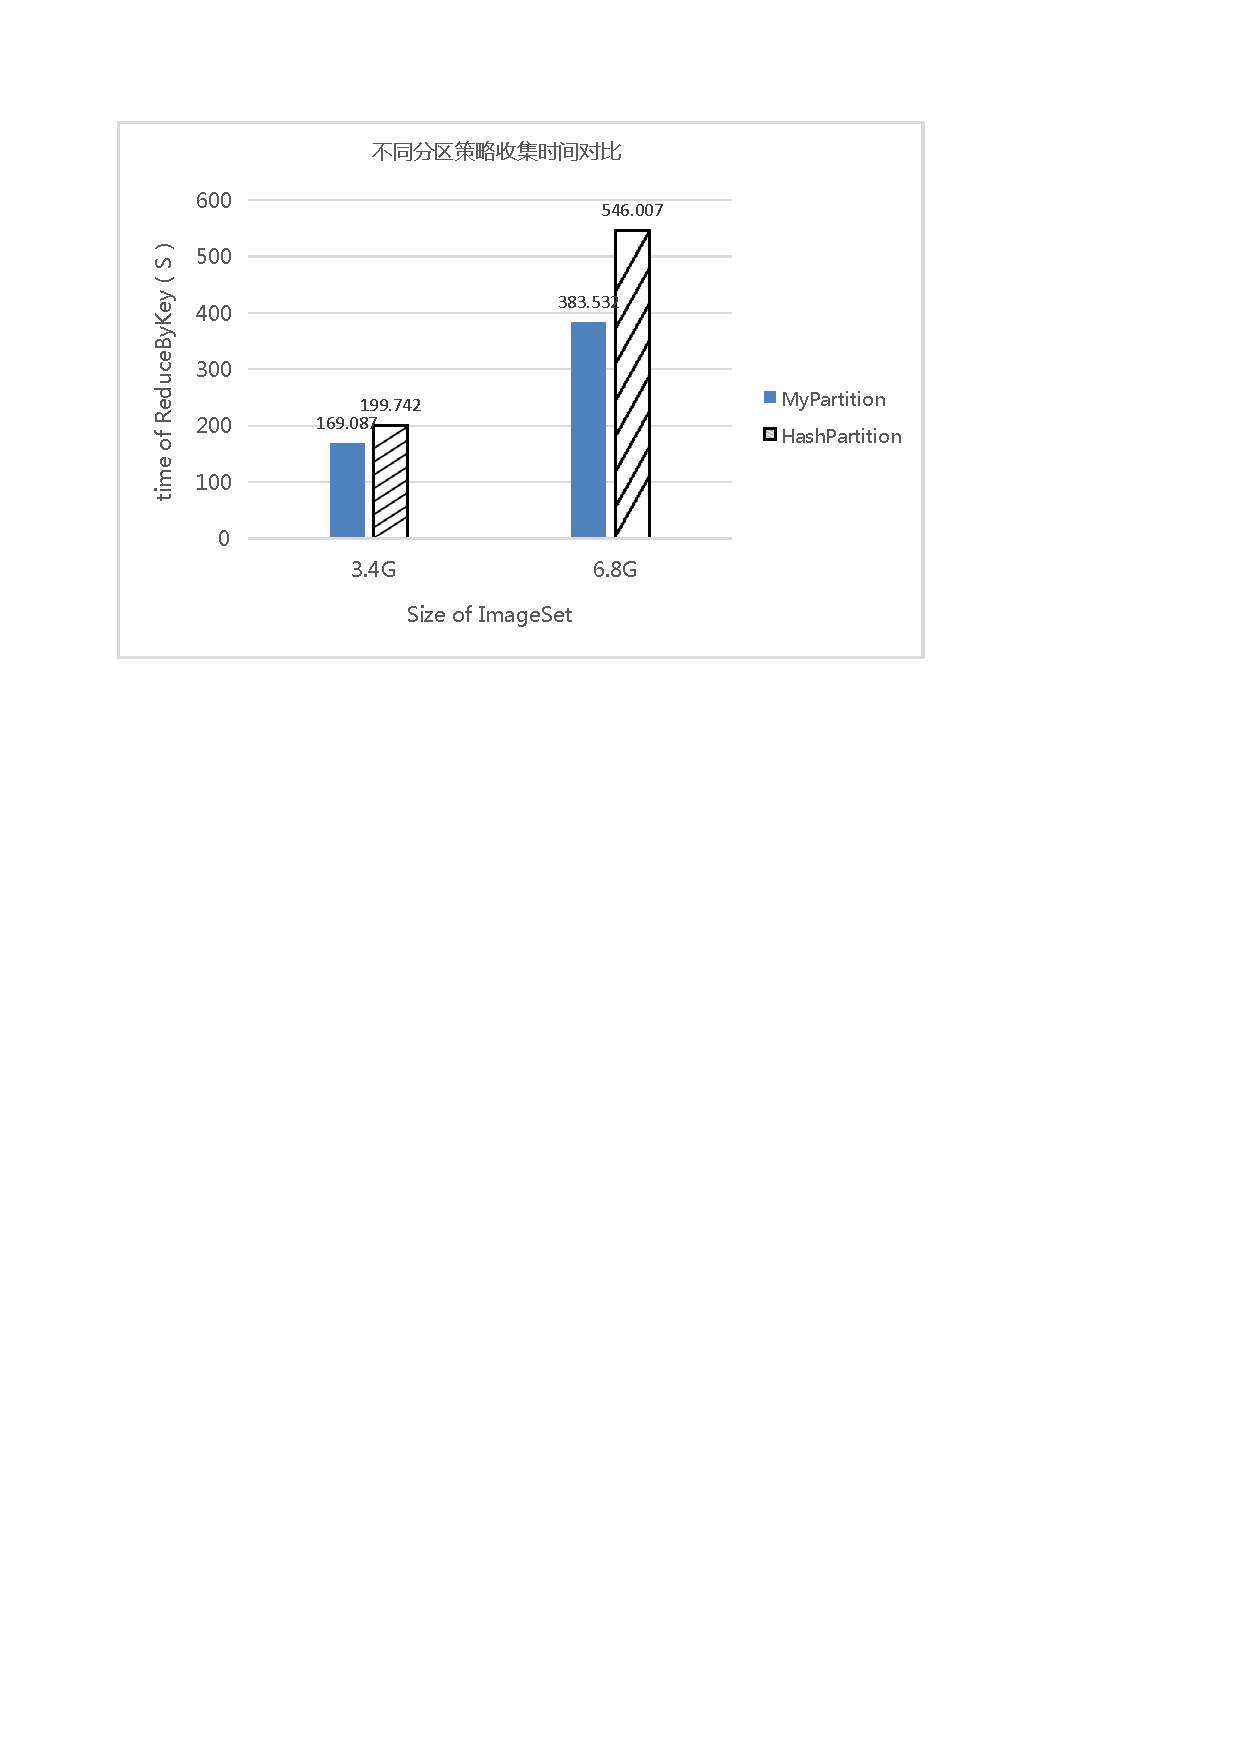
\includegraphics[width=148mm,height=84mm]{data_Partition}
\caption{两种分区策略在收集子块的时间开销}
\label{fig:data_Partition}
\end{figure}

\subsection{系统综合性能对比}
从图\ref{fig:data_fourWays}可以看出,对于500KB的图片集,GPU的处理时间最短,在不到1s的时间就完成了所有图片的特征提取;无论是否采用序列化,Spark-SIFT的特征提取速度比单机还要慢,这是因为在图片数较少时,Spark进行任务分配和数据收集等操作的开销占据了总运行时间中的很大一部分,此时无法体现出Spark的性能优势。当图片集大小为70MB 时,Spark-SIFT的特征速度已经优于单机版本了,序列化方式下的提取时间为44.8s,而单机的提取时间则为470.71s,获得了大约10.5倍的性能加速。GPU版本的处理时间为44.98s,与序列化Spark-SIFT基本相同。随着图片集大小的不断增加,Spark-SIFT在提取时间上的优势也越来越明显。例如,在4GB的输入规模下,Spark-SIFT的处理时间为1319.25s,单机版本的处理时间为28020.03s,处理时间接近Spark-SIFT的20倍,GPU 版本的处理时间为2671.18s,是Spark-SIFT的两倍。因此,对于GB级别以上的图片规模,Spark-SIFT体现出较大的性能优势。
\begin{figure}[htp]
\centering
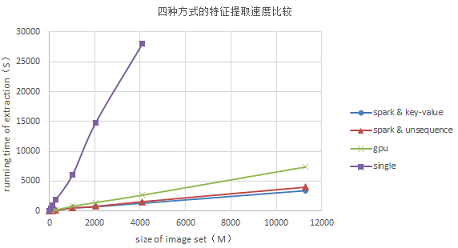
\includegraphics[width=148mm,height=84mm]{data_fourWays}
\caption{四种方式的特征提取速度比较}
\label{fig:data_fourWays}
\end{figure}

总的说来,当图片集大小为GB量级时,与单机版本相比,Spark-SIFT能够带来大约21倍的性能加速,相对于GPU版本能带来大约10倍的性能加速,如图\ref{fig:data_seg_speedup} 所示。
\begin{figure}[htp]
\centering
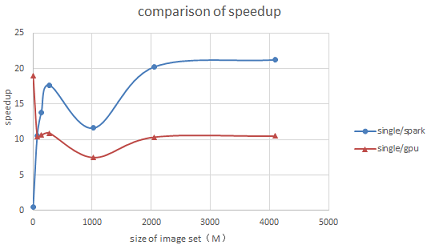
\includegraphics[width=148mm,height=84mm]{data_seg_speedup}
\caption{spark和单机,GPU和单机加速度比较}
\label{fig:data_seg_speedup}
\end{figure}

图\ref{fig:data_spark_gpu}进一步对比了Spark-SIFT 与GPU两个版本的性能,分析了访问磁盘的开销对处理时间的影响。如果没有将结果写到文件中,GPU版本的提取速度快于Spark-SIFT,快了大约0.5倍;当要将结果保存在文件中时,GPU版本的提取速度比Spark-SIFT 慢了约1倍。由此可见,访问磁盘的开销在大规模特征提取时还是相当大的。
\begin{figure}[htp]
\centering
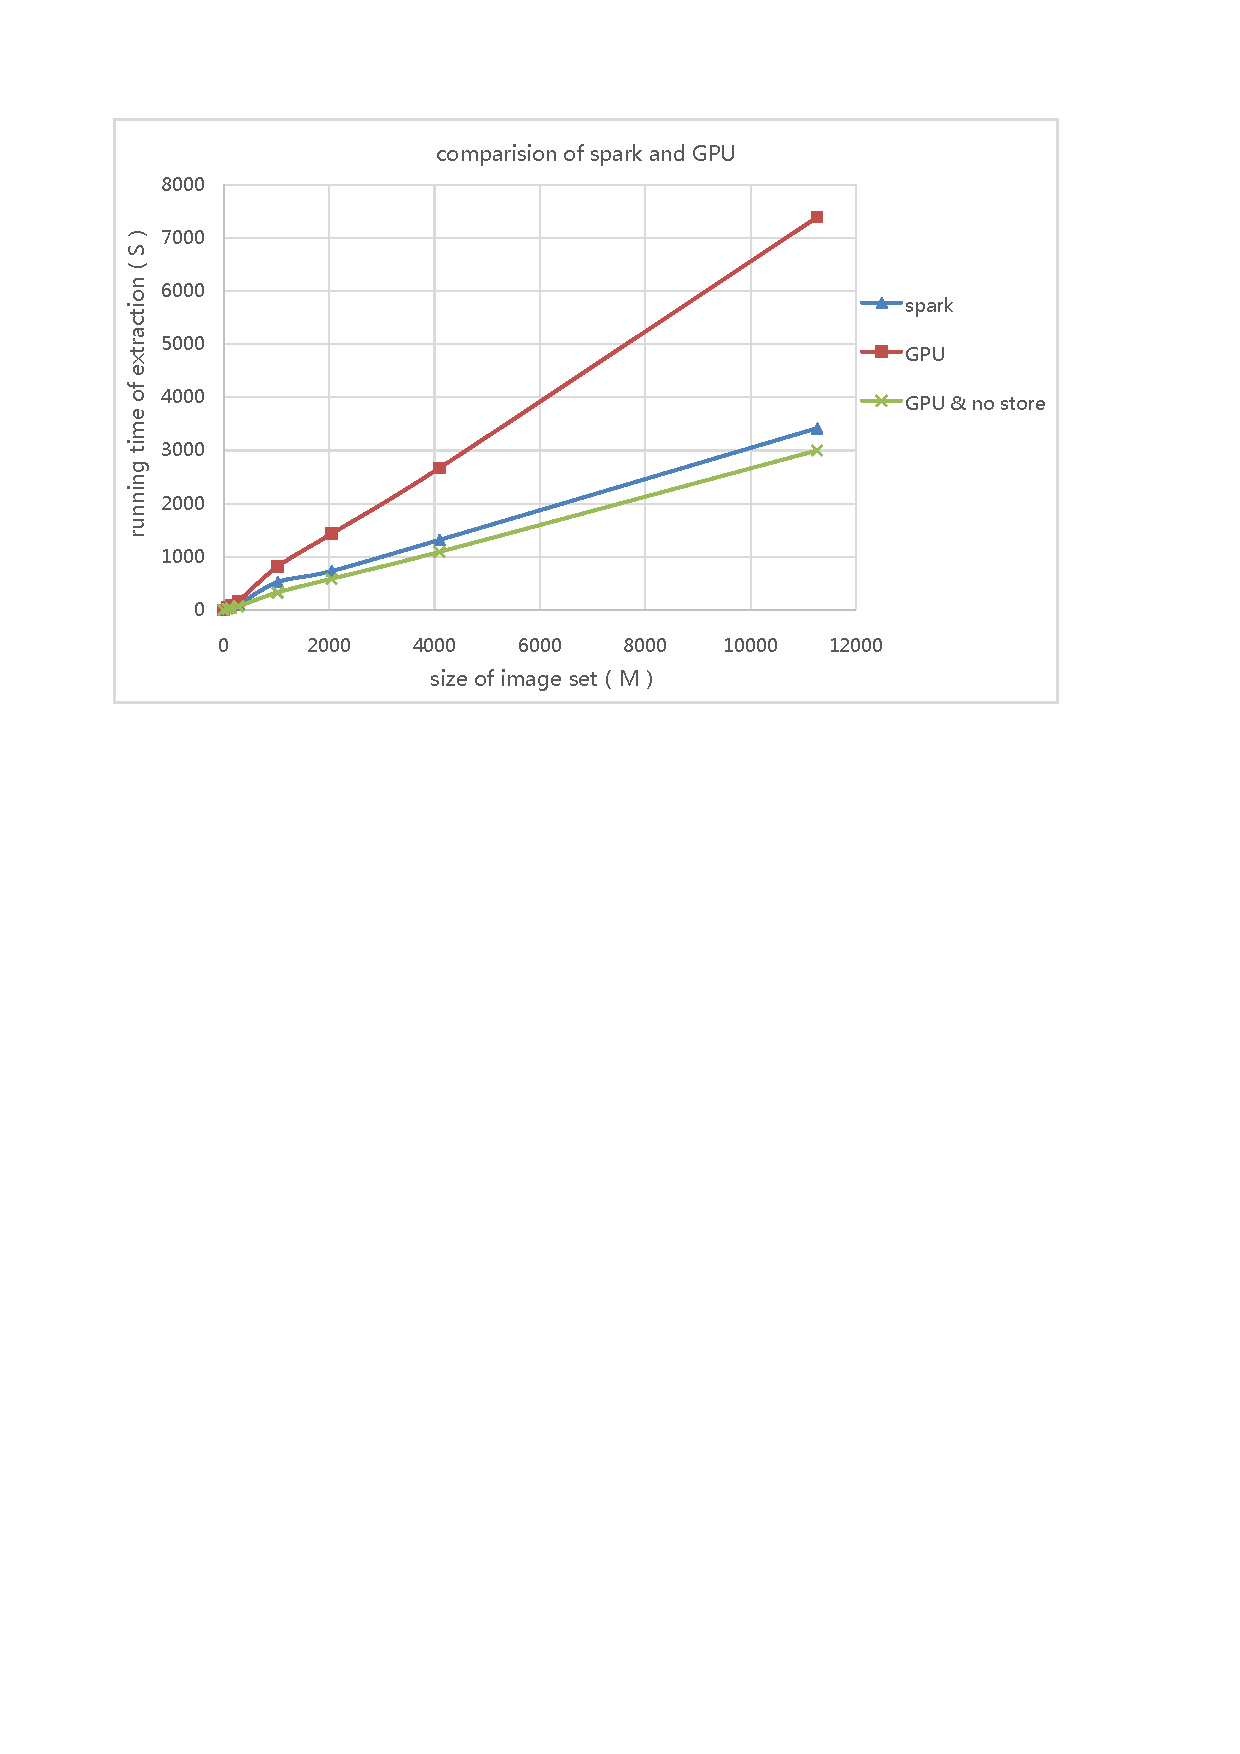
\includegraphics[width=148mm,height=84mm]{data_spark_gpu}
\caption{spark和GPU两种方式比较}
\label{fig:data_spark_gpu}
\end{figure}
\section{本章小结}
本章分析Spark-SIFT系统的综合性能以及针对其提出的三种优化方案。从实验数据来,Spark-SIFT系统在处理GB级别以上的图片数据集时,速度明显快于单机的处理速度,加速比优化GPU,从而达到了设计的预期目标。


\chapter{总结和展望}
\section{全文总结}
随着大数据的不断发展,我们被越来越多的数字信息包围,如何快速的处理海量的数据逐渐成为研究的热点,比如基于图像内容的检索技术就是在该背景下发展成为研究热点,因为现在互联网上的图片越来越多,传统的基于文本的检索技术已不能应对在海量数据中准确检索的要求了。于是本文选取了图像内容检索技术中的最重要步骤特征提取技术作为研究点,研究海量图像库的快速准确特征提取技术。本文的工作可以归纳为以四点:
\begin{compactenum}
\item 设计了一个基于Spark的大规模特征提取系统Spark-SIFT。本文选取了特征提取中具有划时代意义的算法SIFT算法作为Spark下的特征提取算法,该算法精度高,并且具有局部不变性,在目标图片被遮挡或者旋转的情况下依然可以被识别,但是该算法时间复杂度高,实时性差,于是本文根据之前研究者对SIFT算法优化的思路,提出了使用Spark进行SIFT算法加速的设计思路。首先,本文在Spark上设计了一个图像处理的基础库Spark-imageLib,该库提供了图像的表示,图像的常用基础操作等,然后基于该Spark-imageLib 库,本文设计了Spark-sift算法,最后在Spark应用程序中调用Spark-sift算法,进行大规模的图像特征提取;
\item 针对Spark-SIFT系统的加载处理图片低效问题,本文提出了Key-Value的图片描述数据结构。因为现在互联网下图片的体积普遍较小,Spark在加载众多小图片时,会有频繁的磁盘IO 操作,加载的效率比较低。于是,本文提出了一个以key-value描述图片的数据结构,将单张图片转化为一条记录,记录的key为文件名,value为图片的内容字节流,然后将众多的记录序列化保存到HDFS中,之后Spark在加载时就可以一次性加载大量的记录,从而提高了Spark加载处理图片的效率;
\item 针对Spark-SIFT系统的负载不均衡问题,本文提出了分割式特征提取算法。Spark-SIFT在进行特征提取时,我们发现Spark在处理图片大小差异较大的数据集时,会出现负载不均衡的现象,这是由于Spark在任务划分时只考虑了任务的总体积,忽略了图片尺度对任务运行时间的影响。于是本文提出了分割式的特征提取算法,将图片划分为子块,在各个子块上进行特征提取,最后归并在一起。实验数据表明分割式特征提取算法即提高了处理的并行度也解决了负载均衡的问题;
\item 针对分割式算法中存在的Shuffle操作,提供一种Shuffle-Efficient的特征提取算法。因为分割式提取算法虽然提高了并行度,但是也将Shuffle操作引进来了,Shuffle操作会带来频繁的磁盘IO和网络传输开销,十分影响性能。因此,本文提出了高效的分区划分策略,对子块的key值的`\#`字符前的字符串求哈希值,再根据哈希值对分区总数的求余值得到分区号,通过这种方法,使得同一图片的子块散落在同一分区上,从而减少了跨分区收集子块的网络开销;
\end{compactenum}
\section{未来工作展望}
随着4K,8K技术的发展,往后的图片的体积会越来越大,传统的技术技术肯定会面临着许多的问题,我们会对Spark下4K,8K图像处理问题展开研究。同时,我们也会在本文的基础上进行图像内容检索的研究,尝试将大规模的图像库的提取和匹配工作结合一起。最后,因为视频是由一帧帧图片组成的,因此Spark下如何高效进行视频处理也是一个值得深入研究的问题。


%%% Local Variables:
%%% mode: latex
%%% TeX-master: "../main"
%%% End:

\begin{ack}
在论文完成之际,我想对在我求学路上帮助过我,引导过我,关心过我的父母,老师,同学和朋友们致以由衷的感谢! 

感谢我的导师沈立老师,沈老师在我的研究生阶段给了我很大的帮助。刚进入研究生时候,研究生和本科学习上的差异是使得我感到迷茫,沈老师在这时候帮我规划好科研方向,制定好目标,使得我逐渐的适应研究生的生活和学习。之后,沈老师不断的带领我们进行科研攻关,教会我们如何发现问题,怎样去思考问题,在组会上,沈老师总是能抓住问题的要害,分析出问题的根本,在沈老师的带领下,我的科研能力不断提高,逐渐体会到科研的快乐。进入课题之后,沈老师不断的和我讨论课题的方向,帮助我制定好课题的方向,之后沈老师严格的监督我课题的进展,耐心的指导我解决课题中的难题,在沈老师的帮助下,我的课题按照预定目标顺利完成。整个研究生阶段,我在沈老师的悉心指导下,综合素质得到了很大的提高,所以再次向沈老师表示衷心的感谢!

感谢于齐师兄,于齐师兄在我进入实验室后,一直都给予我帮助。于齐师兄为人厚道,热心帮助别人,在我遇到困难的时候,师兄总是向我伸出援手,帮助我解决问题。感谢同队的张万新师兄,万新师兄在我的硕士课题上给予我很大的帮助,在我遇到困惑时,师兄总是不厌其烦的给我讲解,直到我的困惑被彻底解决。感谢钱程师兄,王博千师兄,王璐师姐,徐叶茂师兄,李宁师兄,陈静玮师姐,感谢你们对我的帮助和关怀!

感谢同级同学的刘文杰,番丝江,何锡明,和你们在一起的日子里,我过得十分开心,你们的存在使得我的研究生生涯充满了欢乐!感谢李临同学,和你一块参加比赛,战斗的日子里,我留下了许多美好的回忆!

感谢张诗琴师妹,杨耀华师弟,感谢你们对我课题上的帮助!

感谢我的父母,他们在我常长的路上付出了无比的艰辛,父母用他们辛勤的劳作换来了我现在安逸的生活。感谢我的伯父,他在人生路上给予了我很大帮助,伯父坚韧的性格一直是我学习的榜样。感谢我的大姐,大姐在我成长的路上给了我很大的帮助,无论是在学习上,工作上还是生活上,姐姐总是不断的鼓励我,帮助我,关怀我。家人,你们无条件的爱是我强大的后盾!

最后,感谢在预审,评阅及答辩过程中对我论文提出宝贵意见的给我专家与老师!
\end{ack}


\cleardoublepage
\phantomsection
\addcontentsline{toc}{chapter}{参考文献}
\bibliographystyle{bstutf8}
\bibliography{ref/refs}

\begin{resume}

  \section*{发表的学术论文} % 发表的和录用的合在一起

  \begin{enumerate}[{[}1{]}]
  \addtolength{\itemsep}{-.36\baselineskip}%缩小条目之间的间距,下面类似
  \item Zhang xinming, Yang yaohua, Shen Li, Spark-SIFT:A Spark-Based Large-Scala Image Feature Extract System, SKG2017.
  \end{enumerate}

  \section*{学科竞赛成果} % 有就写,没有就删除
  \begin{enumerate}[{[}1{]}]
  \addtolength{\itemsep}{-.36\baselineskip}%
  \item 2017华为软件精英挑战赛武长赛区一等奖;
  \item 2016三一重工校园APP设计大赛冠军;
  \item 2016华为软件精英挑战赛武长赛区二等奖;
  \end{enumerate}
\end{resume}

% 最后,需要的话还要生成附录,全文随之结束。
\appendix
\backmatter
%%% TeX
\chapter{模板提供的希腊字母命令列表}

大写希腊字母:
\begin{table}[htbp]
\centering
\begin{tabular}{llll}
\toprule
$\Gamma$~\verb|\Gamma| & $\Lambda$~\verb|\Lambda| & $\Sigma$~\verb|\Sigma| & $\Psi$~\verb|\Psi| \\
$\Delta$~\verb|\Delta| & $\Xi$~\verb|\Xi| & $\Upsilon$~\verb|\Upsilon| & $\Omega$~\verb|\Omega| \\
$\Theta$~\verb|\Theta| & $\Pi$~\verb|\Pi| & $\Phi$~\verb|\Phi| & \\
\midrule
$\varGamma$~\verb|\varGamma| & $\varLambda$~\verb|\varLambda| & $\varSigma$~\verb|\varSigma| & $\varPsi$~\verb|\varPsi| \\
$\varDelta$~\verb|\varDelta| & $\varXi$~\verb|\varXi| & $\varUpsilon$~\verb|\varUpsilon| & $\varOmega$~\verb|\varOmega| \\
$\varTheta$~\verb|\varTheta| & $\varPi$~\verb|\varPi| & $\varPhi$~\verb|\varPhi| & \\
\bottomrule
\end{tabular}
\end{table}

小写希腊字母:
\begin{table}[htbp]
\centering
\begin{tabular}{llll}
\toprule
$\alpha$~\verb|\alpha| & $\theta$~\verb|\theta| & $o$~\verb|o| & $\tau$~\verb|\tau| \\ 
$\beta$~\verb|\beta| & $\vartheta$~\verb|\vartheta| & $\pi$~\verb|\pi| & $\upsilon$~\verb|\upsilon| \\ 
$\gamma$~\verb|\gamma| & $\iota$~\verb|\iota| & $\varpi$~\verb|\varpi| & $\phi$~\verb|\phi| \\ 
$\delta$~\verb|\delta| & $\kappa$~\verb|\kappa| & $\rho$~\verb|\rho| & $\varphi$~\verb|\varphi| \\ 
$\epsilon$~\verb|\epsilon| & $\lambda$~\verb|\lambda| & $\varrho$~\verb|\varrho| & $\chi$~\verb|\chi| \\ 
$\varepsilon$~\verb|\varepsilon| & $\mu$~\verb|\mu| & $\sigma$~\verb|\sigma| & $\psi$~\verb|\psi| \\ 
$\zeta$~\verb|\zeta| & $\nu$~\verb|\nu| & $\varsigma$~\verb|\varsigma| & $\omega$~\verb|\omega| \\ 
$\eta$~\verb|\eta| & $\xi$~\verb|\xi| & $\varkappa$~\verb|\varkappa| & $\digamma$~\verb|\digamma| \\ 
\midrule
$\upalpha$~\verb|\upalpha| & $\uptheta$~\verb|\uptheta| & $\mathrm{o}$~\verb|\mathrm{o}| & $\uptau$~\verb|\uptau| \\ 
$\upbeta$~\verb|\upbeta| & $\upvartheta$~\verb|\upvartheta| & $\uppi$~\verb|\uppi| & $\upupsilon$~\verb|\upupsilon| \\ 
$\upgamma$~\verb|\upgamma| & $\upiota$~\verb|\upiota| & $\upvarpi$~\verb|\upvarpi| & $\upphi$~\verb|\upphi| \\ 
$\updelta$~\verb|\updelta| & $\upkappa$~\verb|\upkappa| & $\uprho$~\verb|\uprho| & $\upvarphi$~\verb|\upvarphi| \\ 
$\upepsilon$~\verb|\upepsilon| & $\uplambda$~\verb|\uplambda| & $\upvarrho$~\verb|\upvarrho| & $\upchi$~\verb|\upchi| \\ 
$\upvarepsilon$~\verb|\upvarepsilon| & $\upmu$~\verb|\upmu| & $\upsigma$~\verb|\upsigma| & $\uppsi$~\verb|\uppsi| \\ 
$\upzeta$~\verb|\upzeta| & $\upnu$~\verb|\upnu| & $\upvarsigma$~\verb|\upvarsigma| & $\upomega$~\verb|\upomega| \\ 
$\upeta$~\verb|\upeta| & $\upxi$~\verb|\upxi| & & \\ 
\bottomrule
\end{tabular}
\end{table}

希腊字母属于数学符号类别,请用\verb|\bm|命令加粗,其余向量、矩阵可用\verb|\mathbf|。


\end{document}
